\subsubsection{Full State-Resolution Sensitivity Table}
\label{sec:sensitivity_table}

Table~\ref{tab:sensitivity} reports the full $K$-sweep referenced in Section~\ref{sec:k_selection_results} of the main text.
Observed excess kurtosis is $7.68$ IS and $5.29$ OoS at all $K$.

\begin{table}[H]
\centering
\caption{State resolution sensitivity for SPY CHMM-N (1{,}000 paths, $\alpha = 0.05$). Every metric is computed on the identical simulation pipeline used for Table~\ref{tab:model_comparison} in the main text. IS coverage was 100\% at every $K$; OoS coverage is reported separately. ACF-MAE columns: $|G_t|$ measures the volatility-clustering reproduction; $G_t$ measures linear-autocorrelation reproduction (parallel to $|G_t|$, both averaged over lags 1--252).}
\label{tab:sensitivity}
\small
\begin{tabular}{c cc cc cc cc c c c}
\toprule
& \multicolumn{2}{c}{KS (\%)} & \multicolumn{2}{c}{AD (\%)} & \multicolumn{2}{c}{Kurtosis} & \multicolumn{2}{c}{ACF-MAE} & & & \\
\cmidrule(lr){2-3} \cmidrule(lr){4-5} \cmidrule(lr){6-7} \cmidrule(lr){8-9}
$K$ & IS & OoS & IS & OoS & Obs & Sim & $|G_t|$ & $G_t$ & $W_1$ & $H$ & Cov OoS (\%) \\
\midrule
3  & 89.0 & 77.2 & 78.9 & 68.6 & 7.68 & 3.82 & 0.0463 & 0.0240 & 0.131 & 0.0839 & 94.9 \\
6  & 92.9 & 78.7 & 84.3 & 74.3 & 7.68 & 5.38 & 0.0496 & 0.0238 & 0.116 & 0.0829 & 90.9 \\
9  & 93.0 & 81.4 & 84.4 & 74.4 & 7.68 & 4.63 & 0.0492 & 0.0238 & 0.118 & 0.0810 & 91.9 \\
12 & 94.9 & 81.6 & 85.8 & 75.0 & 7.68 & 4.57 & 0.0500 & 0.0238 & 0.113 & 0.0801 & 91.9 \\
15 & 93.9 & 81.0 & 84.8 & 73.5 & 7.68 & 4.89 & 0.0508 & 0.0238 & 0.114 & 0.0804 & 88.9 \\
\textbf{18} & 94.8 & 85.5 & 88.2 & 79.7 & 7.68 & 5.04 & 0.0515 & 0.0237 & 0.110 & 0.0807 & 91.9 \\
21 & \textbf{95.6} & \textbf{88.0} & \textbf{89.1} & \textbf{78.8} & 7.68 & 3.78 & 0.0534 & \textbf{0.0236} & 0.112 & 0.0801 & \textbf{99.0} \\
\bottomrule
\end{tabular}
\end{table}

\subsubsection{Multi-Emission State-Resolution Sensitivity}
\label{sec:multi_emission_sensitivity}

Table~\ref{tab:sensitivity_multi} extends Table~\ref{tab:sensitivity} across the three emission families, confirming that the qualitative operating point $K = 18$ is stable when the Gaussian component is replaced with Student-t or Laplace emissions.
For CHMM-t the per-state degrees of freedom $\nu_k$ are refit by ECM-plus-golden-section at every $K$; for CHMM-L the weighted-median location and weighted MAD scale are closed form and impose no additional cost.
Three patterns extend from Table~\ref{tab:sensitivity} to the new families.
First, the distributional pass rates plateau in the $K \in \{12, 15, 18, 21\}$ band for all three families: CHMM-t reaches its highest IS KS at $K = 18$ ($96.0\%$) and its highest OoS KS at $K = 18$ ($84.5\%$), and CHMM-L reaches its highest IS KS at $K = 18$ ($95.6\%$) and its highest IS AD at $K = 18$ ($92.7\%$).
Once a family enters the plateau the operating point is flat with respect to $K$, so we report the main-text results at the same $K = 18$ used for CHMM-N.
Second, the absolute-return ACF-MAE remains within the narrow $0.047$--$0.056$ band observed for the Gaussian sweep, and the raw-return ACF-MAE remains essentially constant at $\approx 0.024$ across all $21$ (family, $K$) combinations. Both temporal axes are properties of the regime structure rather than the emission family: $|G_t|$ ACF reproduction is governed by the eigenvalue spectrum of $\mathbf T$ (Section~\ref{sec:theory}), and raw-$G_t$ ACF is null in expectation under any HMM with i.i.d.\ within-state emissions.
Third, simulated kurtosis behaves as expected from the component families: the Gaussian sweep peaks around $5.0$ at the high-$K$ end, the Laplace sweep lands squarely in the $5.3$--$6.7$ range (closest to the observed $7.68$), and the Student-t sweep climbs sharply above $13$ across the entire sweep because the ECM search assigns small $\nu_k$ to a subset of tail states, over-correcting IS kurtosis.

\begin{table}[H]
\centering
\caption{Multi-emission state resolution sensitivity for SPY (1{,}000 paths, $\alpha = 0.05$). CHMM-N: Gaussian; CHMM-t: Student-t with per-state $\nu_k$ refit by ECM-plus-golden-section; CHMM-L: Laplace with weighted-median location and weighted-MAD scale. Every metric is computed on the identical simulation pipeline used for Table~\ref{tab:model_comparison}. Observed excess kurtosis is $7.68$ IS and $5.29$ OoS. ACF-MAE columns parallel the main-text Table~\ref{tab:model_comparison}: $|G_t|$ for volatility clustering, $G_t$ (raw) for linear autocorrelation.}
\label{tab:sensitivity_multi}
\small
\resizebox{\textwidth}{!}{%
\begin{tabular}{l c cc cc c cc c c}
\toprule
& & \multicolumn{2}{c}{KS (\%)} & \multicolumn{2}{c}{AD (\%)} & & \multicolumn{2}{c}{ACF-MAE} & & \\
\cmidrule(lr){3-4} \cmidrule(lr){5-6} \cmidrule(lr){8-9}
Family & $K$ & IS & OoS & IS & OoS & Kurt (IS sim) & $|G_t|$ & $G_t$ & $W_1$ IS & $H$ IS \\
\midrule
CHMM-N & 3  & 89.7 & 80.1 & 79.2 & 70.7 & 3.86  & 0.0467 & 0.0240 & 0.128 & 0.0833 \\
       & 6  & 93.8 & 79.1 & 87.2 & 72.8 & 5.29  & 0.0504 & 0.0238 & 0.114 & 0.0825 \\
       & 9  & 94.9 & 83.0 & 84.3 & 74.8 & 4.58  & 0.0490 & 0.0238 & 0.115 & 0.0806 \\
       & 12 & 93.7 & 82.7 & 85.5 & 75.0 & 4.56  & 0.0501 & 0.0237 & 0.115 & 0.0804 \\
       & 15 & 93.6 & 83.0 & 87.0 & 75.1 & 4.89  & 0.0509 & 0.0238 & 0.114 & 0.0803 \\
       & \textbf{18} & 94.7 & 83.4 & 88.5 & 76.6 & 4.97  & 0.0511 & 0.0237 & 0.108 & 0.0805 \\
       & 21 & \textbf{95.1} & \textbf{88.0} & \textbf{88.2} & \textbf{79.7} & 3.80  & 0.0532 & 0.0236 & 0.110 & 0.0796 \\
\midrule
CHMM-t & 3  & 92.2 & 82.9 & 88.0 & 79.1 & 33.68 & 0.0538 & 0.0235 & 0.108 & 0.0759 \\
       & 6  & 91.8 & 80.4 & 86.7 & 74.8 & 22.74 & 0.0527 & 0.0235 & 0.108 & 0.0772 \\
       & 9  & 95.4 & 84.0 & 89.9 & 78.0 & 16.60 & 0.0535 & 0.0234 & 0.102 & 0.0752 \\
       & 12 & 95.2 & 85.0 & 89.8 & 78.4 & 14.98 & 0.0543 & 0.0234 & 0.100 & 0.0757 \\
       & 15 & 94.7 & 83.7 & 88.8 & 79.5 & 16.36 & 0.0539 & 0.0234 & 0.101 & 0.0758 \\
       & \textbf{18} & \textbf{96.0} & \textbf{84.5} & \textbf{91.7} & \textbf{80.8} & 13.19 & 0.0551 & \textbf{0.0234} & \textbf{0.099} & \textbf{0.0759} \\
       & 21 & 94.5 & 83.3 & 88.5 & 78.1 & 14.66 & 0.0539 & 0.0234 & 0.102 & 0.0758 \\
\midrule
CHMM-L & 3  & 81.9 & 64.8 & 82.5 & 65.8 & 5.29  & 0.0535 & 0.0235 & 0.112 & 0.0854 \\
       & 6  & 90.5 & 76.4 & 85.0 & 74.2 & 5.91  & 0.0513 & 0.0235 & 0.110 & 0.0818 \\
       & 9  & 90.5 & 75.7 & 84.8 & 70.1 & 6.01  & 0.0517 & 0.0235 & 0.110 & 0.0819 \\
       & 12 & 93.6 & 81.4 & 89.8 & 78.8 & 6.18  & 0.0541 & 0.0234 & 0.106 & 0.0796 \\
       & 15 & 92.5 & 78.9 & 88.3 & 78.8 & 6.03  & 0.0541 & 0.0234 & 0.105 & 0.0792 \\
       & \textbf{18} & \textbf{95.6} & \textbf{79.9} & \textbf{92.7} & \textbf{80.7} & \textbf{6.74}  & 0.0563 & 0.0234 & 0.101 & 0.0798 \\
       & 21 & 93.1 & 79.5 & 87.7 & 76.8 & 6.05  & 0.0543 & 0.0234 & 0.107 & 0.0807 \\
\bottomrule
\end{tabular}%
}
\end{table}

\subsubsection{Baum-Welch Convergence}
\label{sec:convergence}

Figure~\ref{fig:convergence_all} shows the Baum-Welch convergence curves for representative state resolutions.
All models converged within the 60-iteration budget, with the log-likelihood monotonically increasing (as guaranteed by the EM algorithm).
Lower $K$ values typically converged faster (15--25 iterations), while higher $K$ values required 25--40 iterations to reach the convergence tolerance of $|\Delta\mathcal{L}| < 10^{-4}$.
The monotonic increase confirms that the quantile-based initialization provided a valid starting point from which the EM algorithm could improve without encountering degenerate solutions.

\begin{figure}[H]
\centering
\begin{subfigure}[b]{0.32\textwidth}
    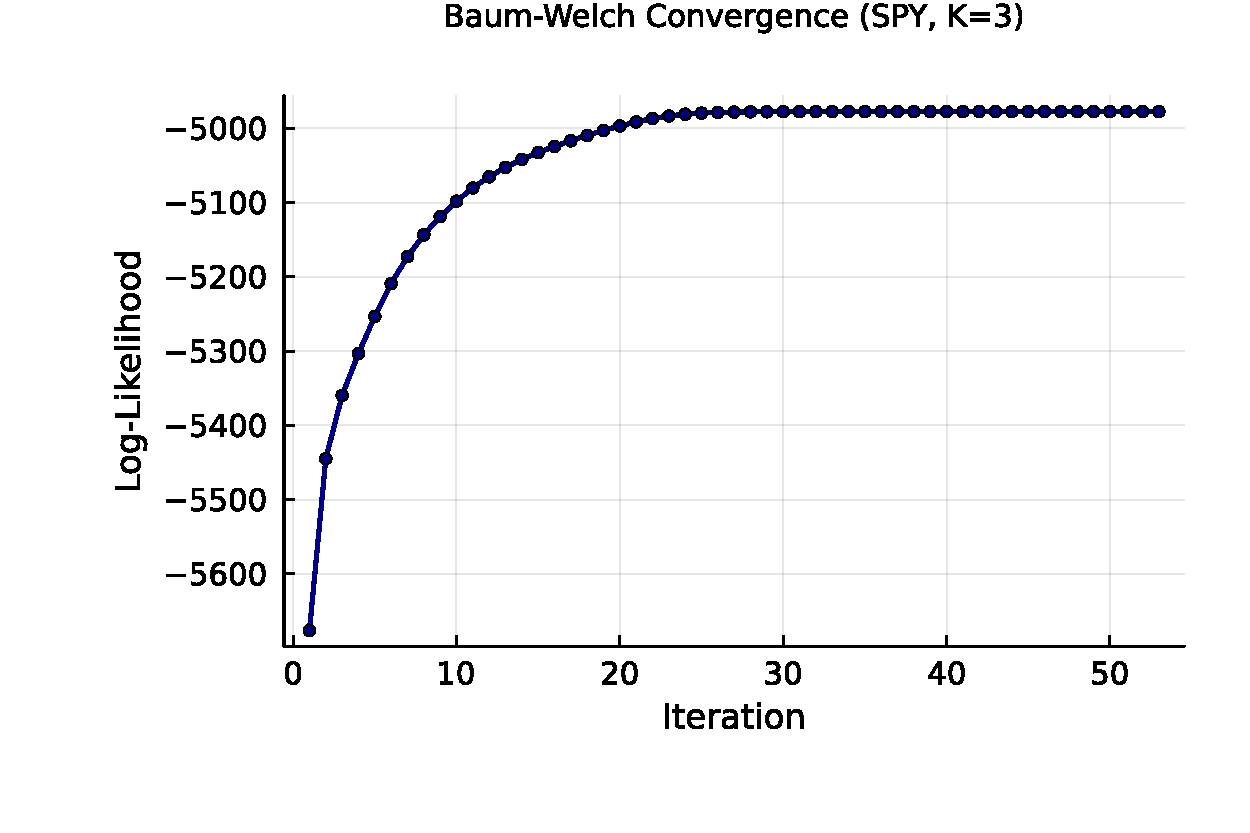
\includegraphics[width=\textwidth]{figs/Fig-Convergence-K3.pdf}
    \caption{$K = 3$}
\end{subfigure}
\hfill
\begin{subfigure}[b]{0.32\textwidth}
    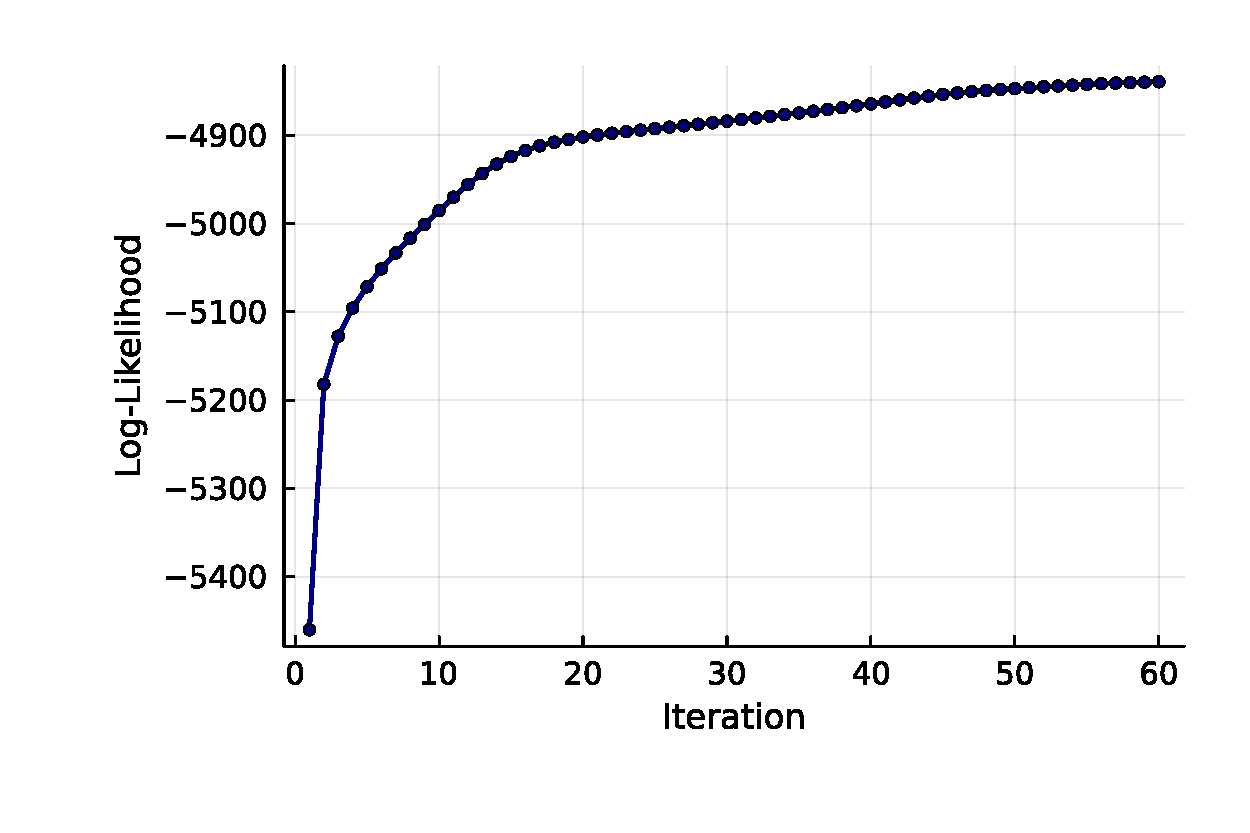
\includegraphics[width=\textwidth]{figs/Fig-Convergence-K12.pdf}
    \caption{$K = 12$}
\end{subfigure}
\hfill
\begin{subfigure}[b]{0.32\textwidth}
    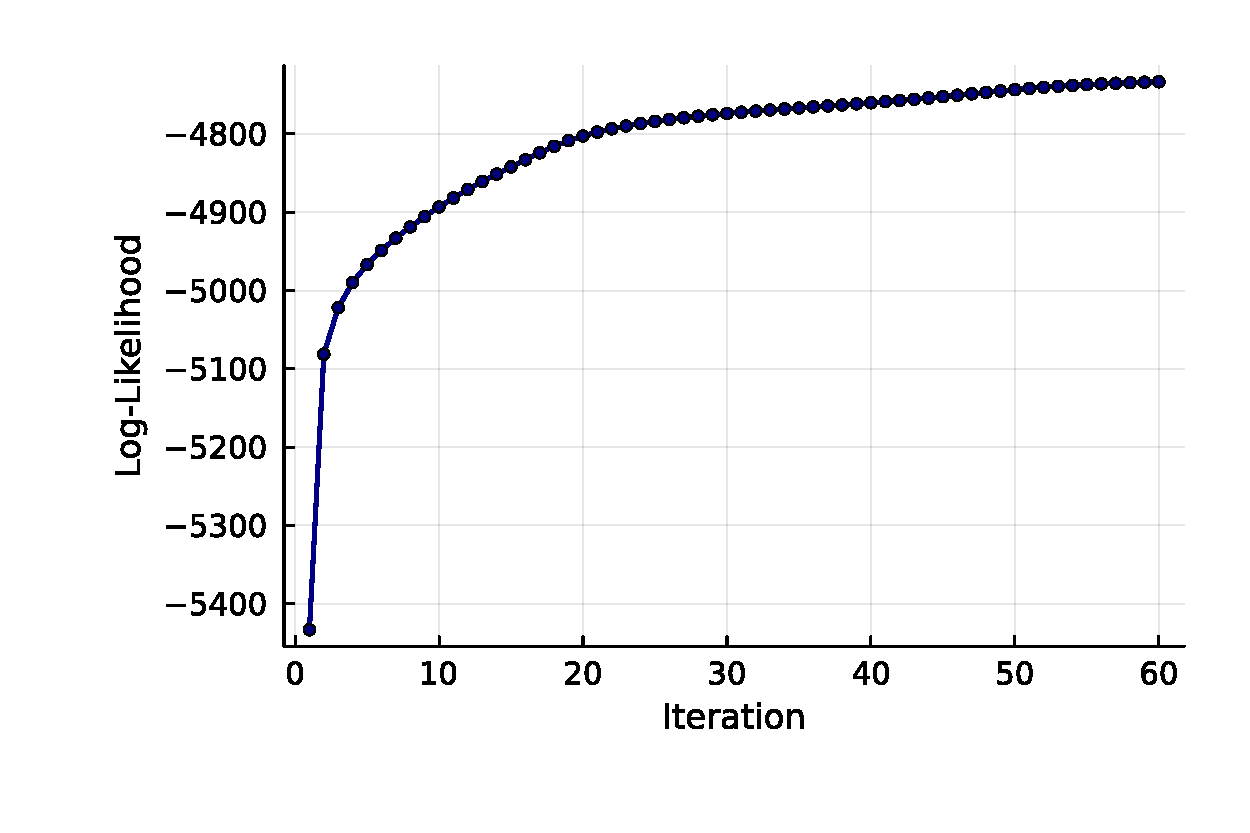
\includegraphics[width=\textwidth]{figs/Fig-Convergence-K18.pdf}
    \caption{$K = 18$ (selected)}
\end{subfigure}
\caption{Baum-Welch convergence for the SPY CHMM-N fit (Pipeline~A, IS) at selected state resolutions. Log-likelihood is monotonically increasing (EM guarantee) and plateaus well before $\texttt{max\_iter} = 60$.}
\label{fig:convergence_all}
\end{figure}

\subsubsection{IS Comparison at Non-Selected State Resolutions}
\label{sec:k_sweep_panels}

Figures~\ref{fig:k_sweep_panels_is}--\ref{fig:k_sweep_is_k21} show the IS model comparison panels for $K \in \{3, 6, 12, 21\}$, complementing the $K = 18$ comparison in Figure~\ref{fig:is_comparison} of the main text.
Across all resolutions, the CHMM's simulated density closely overlays the observed density, and the ACF of absolute returns tracks the slow decay pattern.
The visible improvement from $K = 3$ to $K = 18$ is concentrated in the tails of the Q-Q panel and the steady-state level of the ACF panel.
$K = 9$ and $K = 15$ panels are omitted because they interpolate smoothly between the shown resolutions; their numerical metrics are in Table~\ref{tab:sensitivity}.

\begin{figure}[H]
\centering
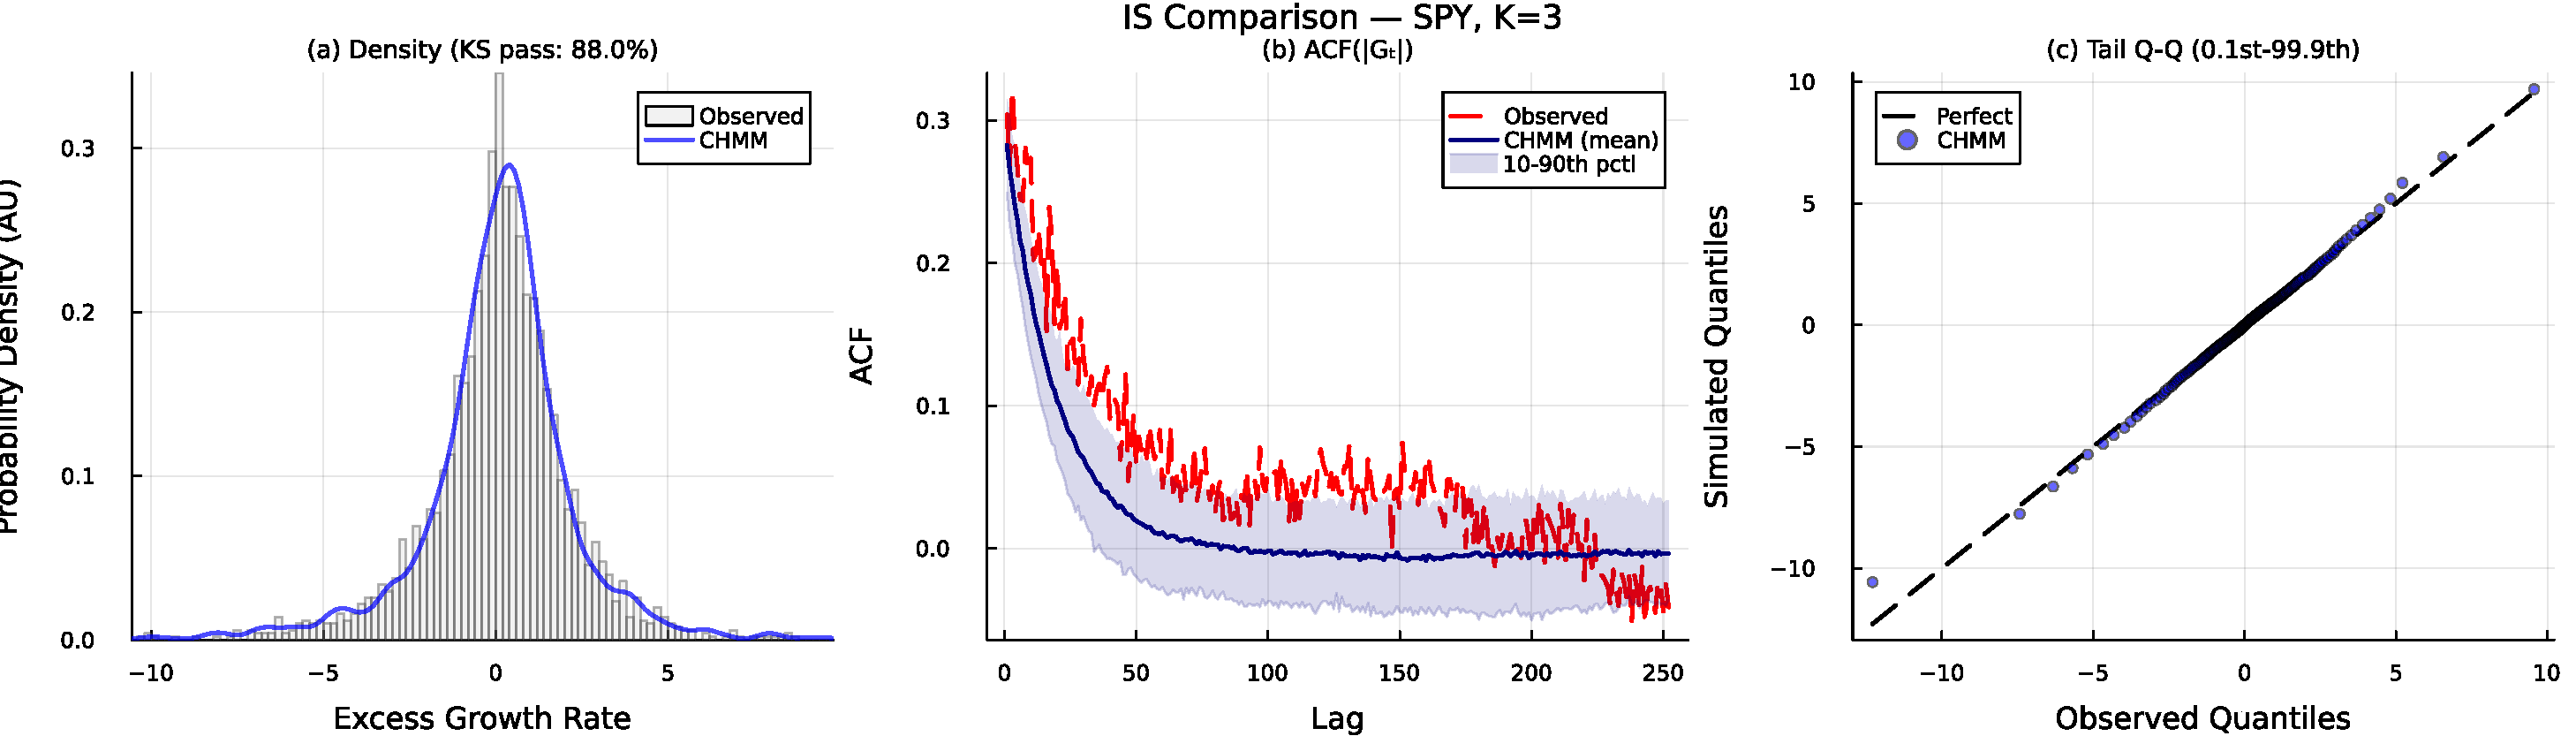
\includegraphics[width=\textwidth]{figs/Fig-3-IS-Comparison-K3.pdf}
\caption{IS SPY CHMM-N comparison at $K = 3$ (Pipeline~A, 1{,}000 simulated paths; panels as in Figure~\ref{fig:is_comparison}). The $K = 18$ counterpart is Figure~\ref{fig:is_comparison} of the main text.}
\label{fig:k_sweep_panels_is}
\end{figure}

\begin{figure}[H]
\centering
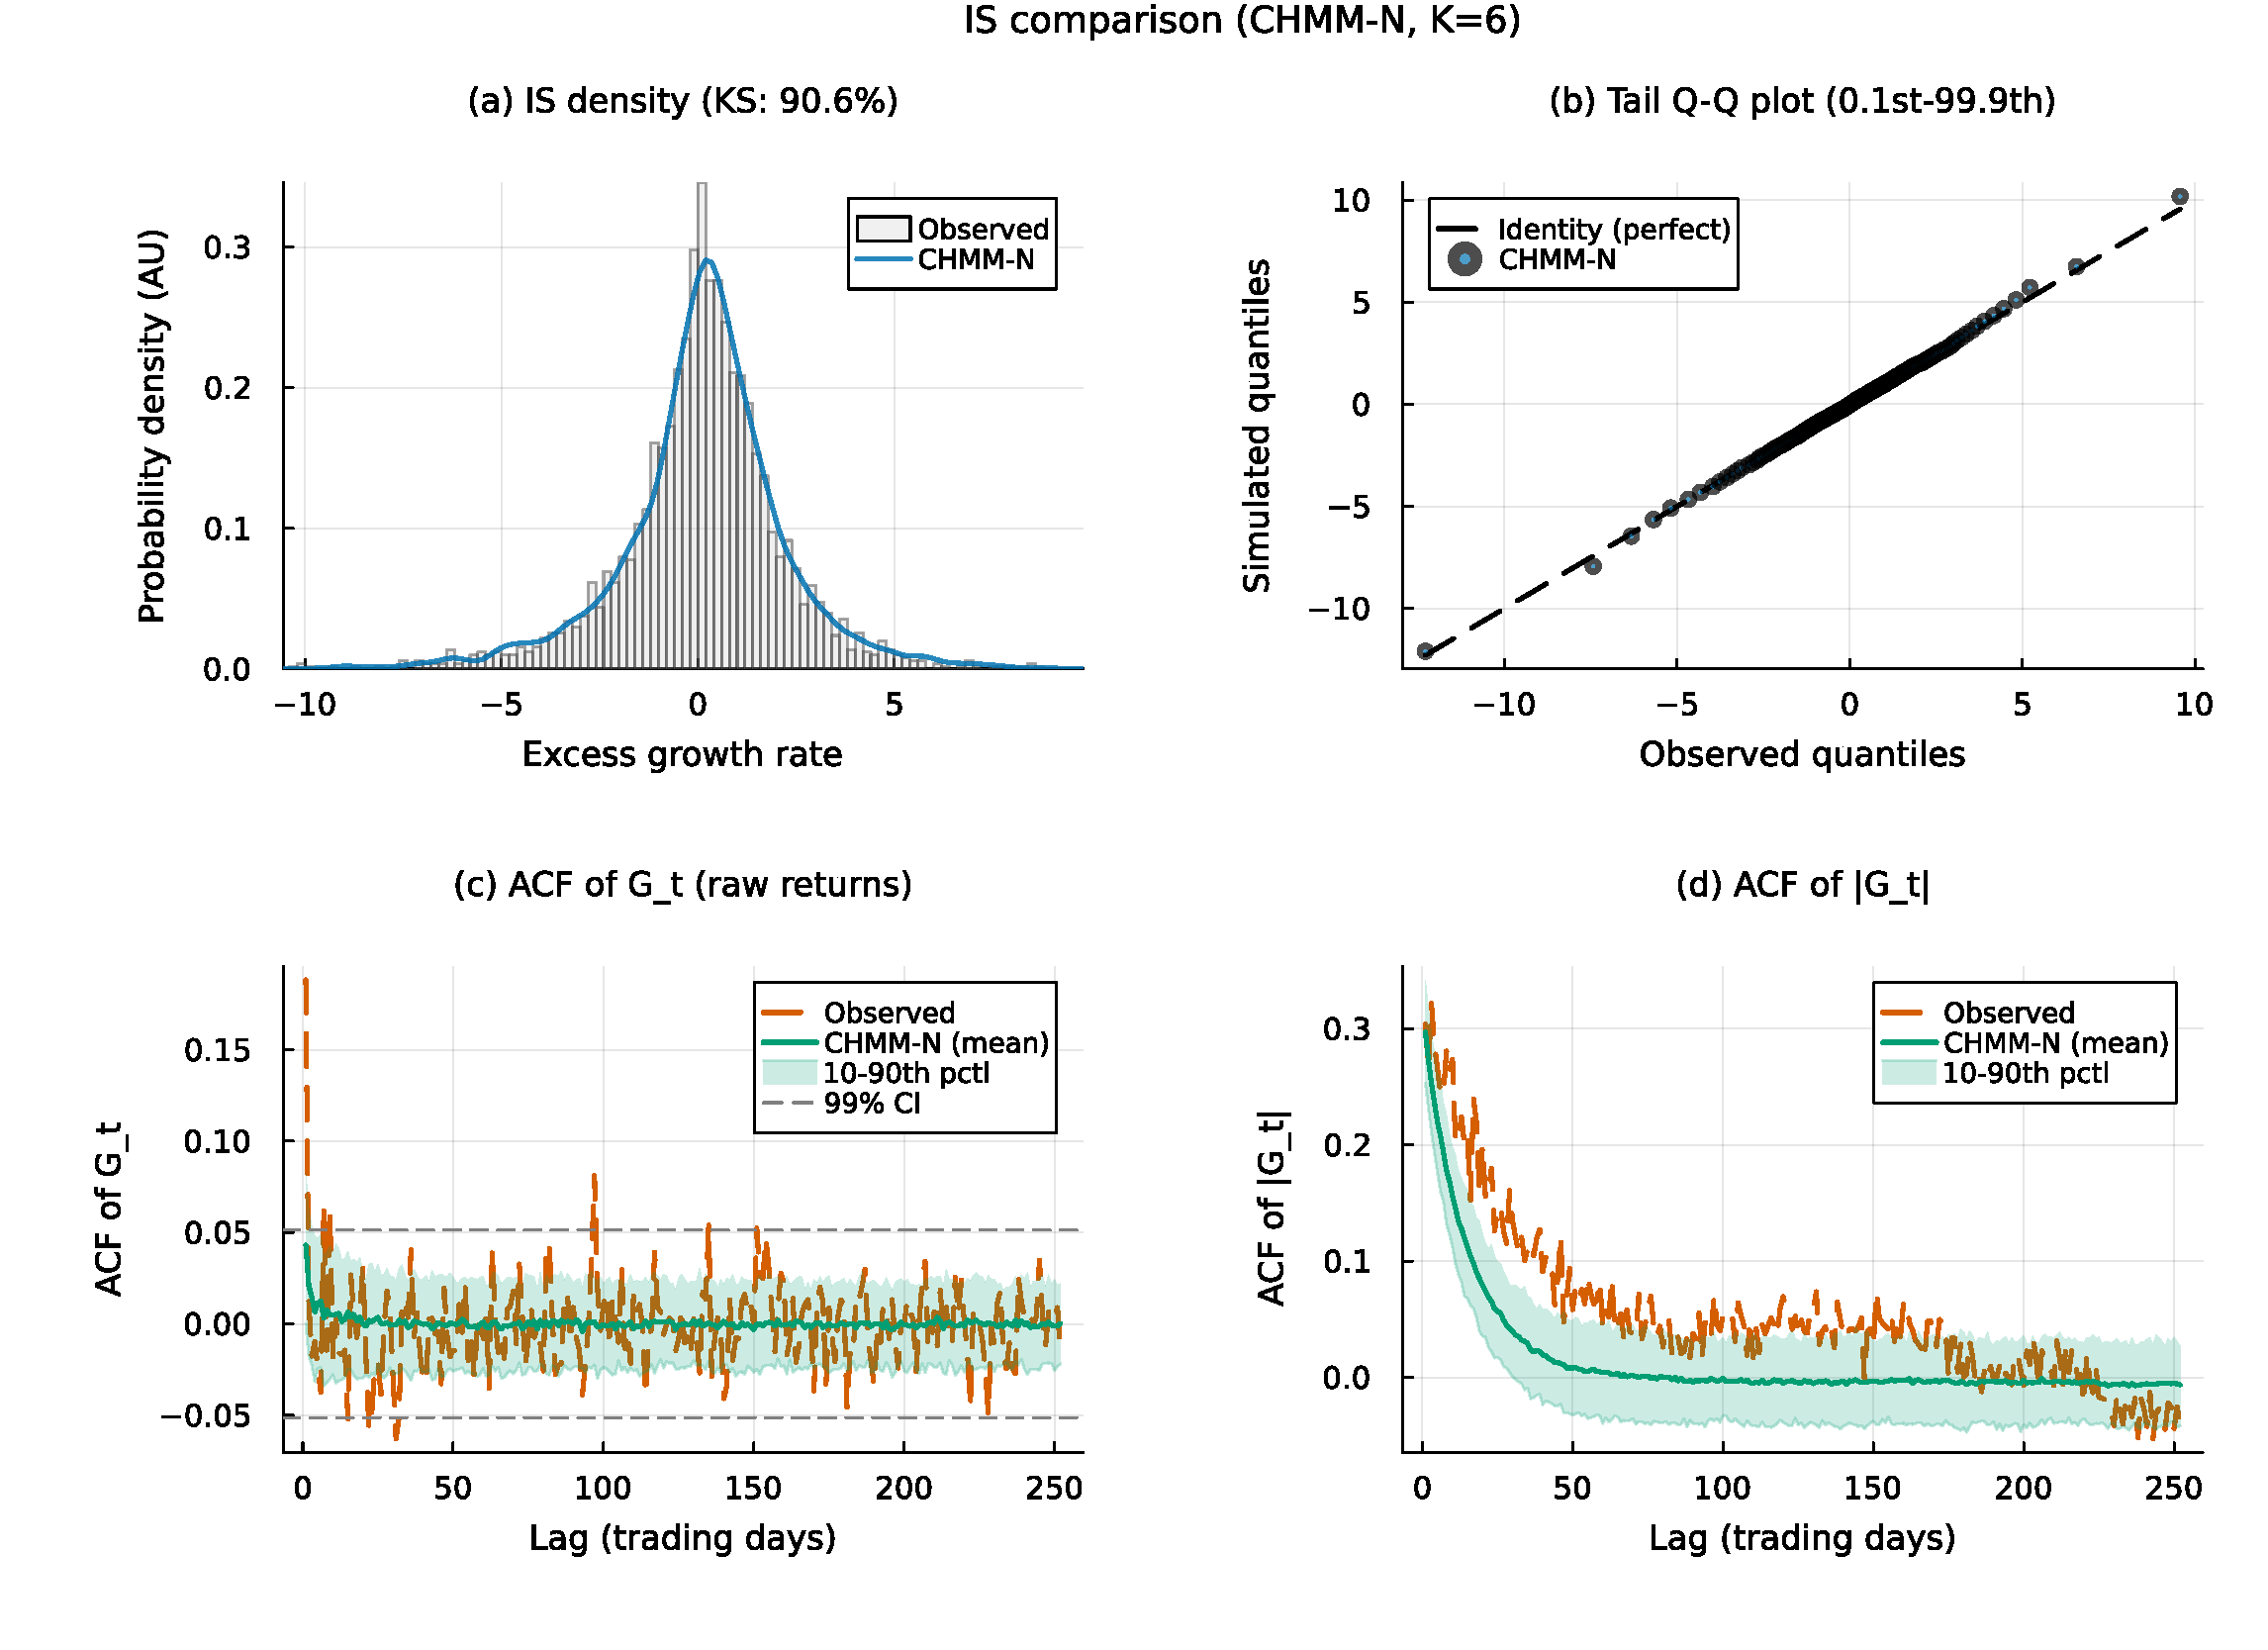
\includegraphics[width=\textwidth]{figs/Fig-3-IS-Comparison-K6.pdf}
\caption{IS SPY CHMM-N comparison at $K = 6$ (Pipeline~A, 1{,}000 simulated paths; panels as in Figure~\ref{fig:is_comparison}).}
\label{fig:k_sweep_is_k6}
\end{figure}

\begin{figure}[H]
\centering
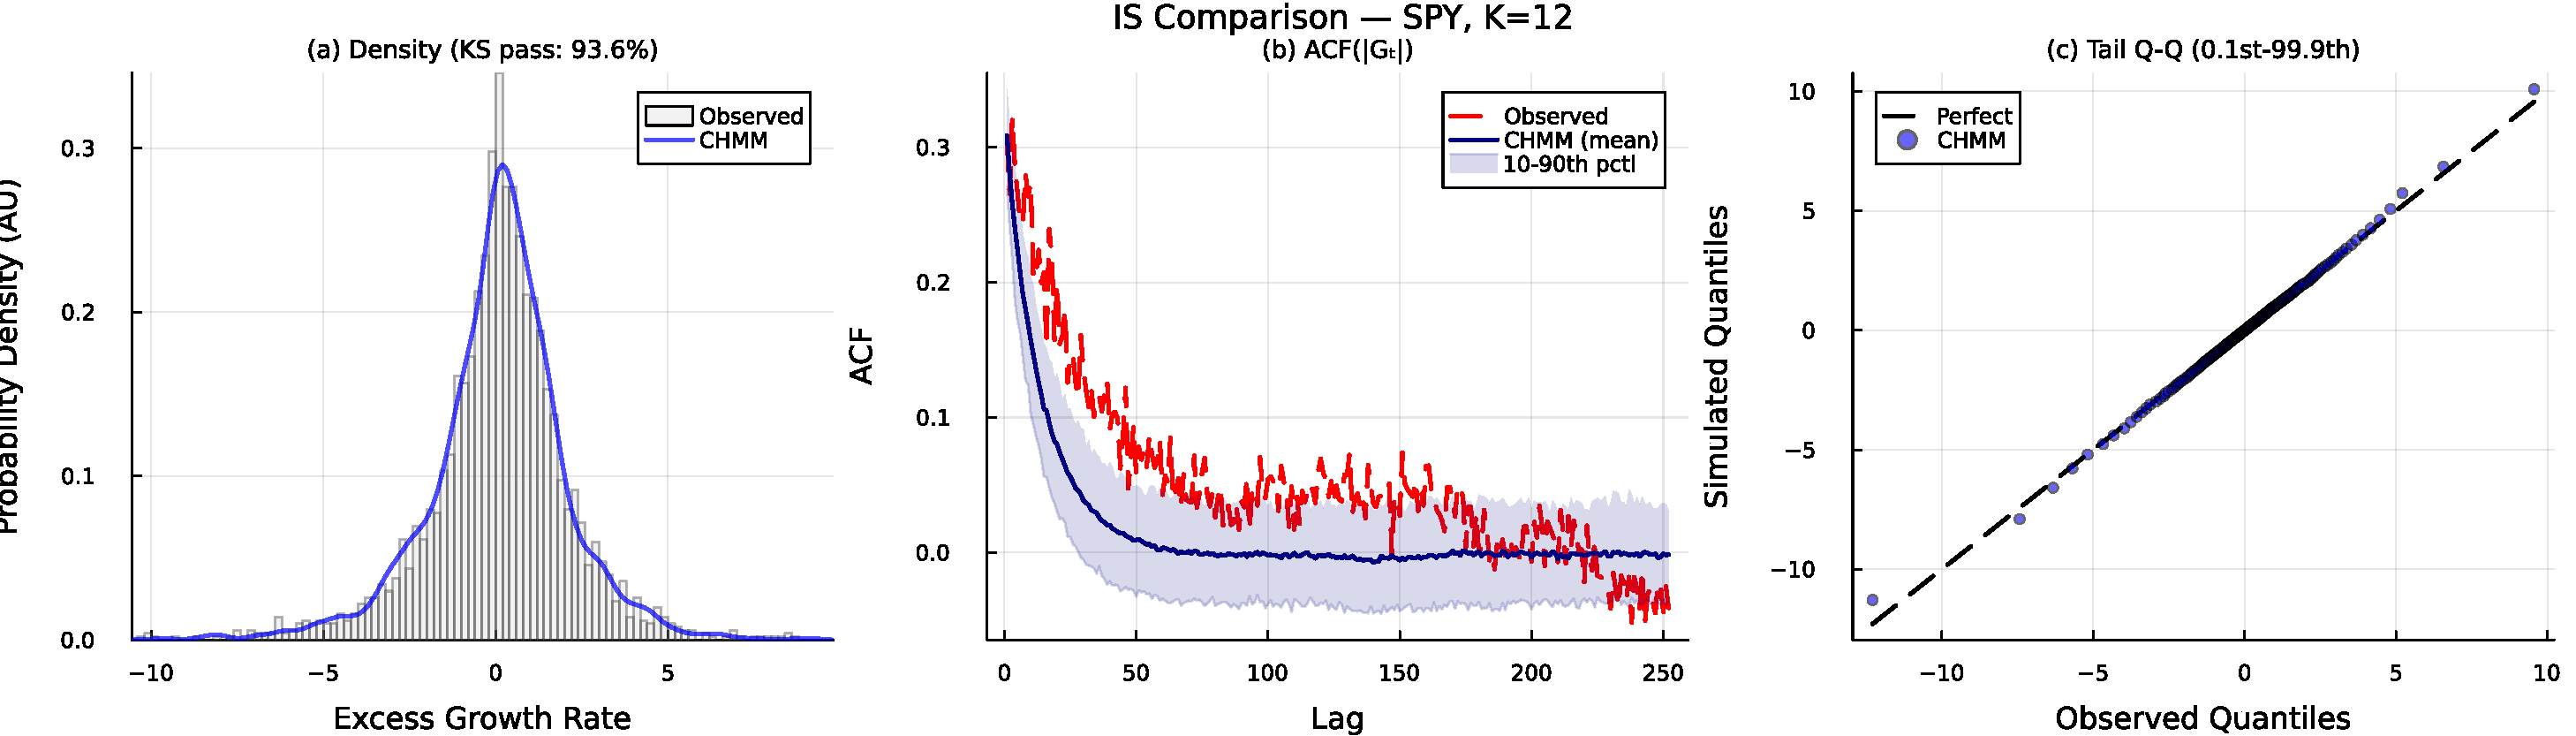
\includegraphics[width=\textwidth]{figs/Fig-3-IS-Comparison-K12.pdf}
\caption{IS SPY CHMM-N comparison at $K = 12$ (Pipeline~A, 1{,}000 simulated paths; panels as in Figure~\ref{fig:is_comparison}).}
\label{fig:k_sweep_is_k12}
\end{figure}

\begin{figure}[H]
\centering
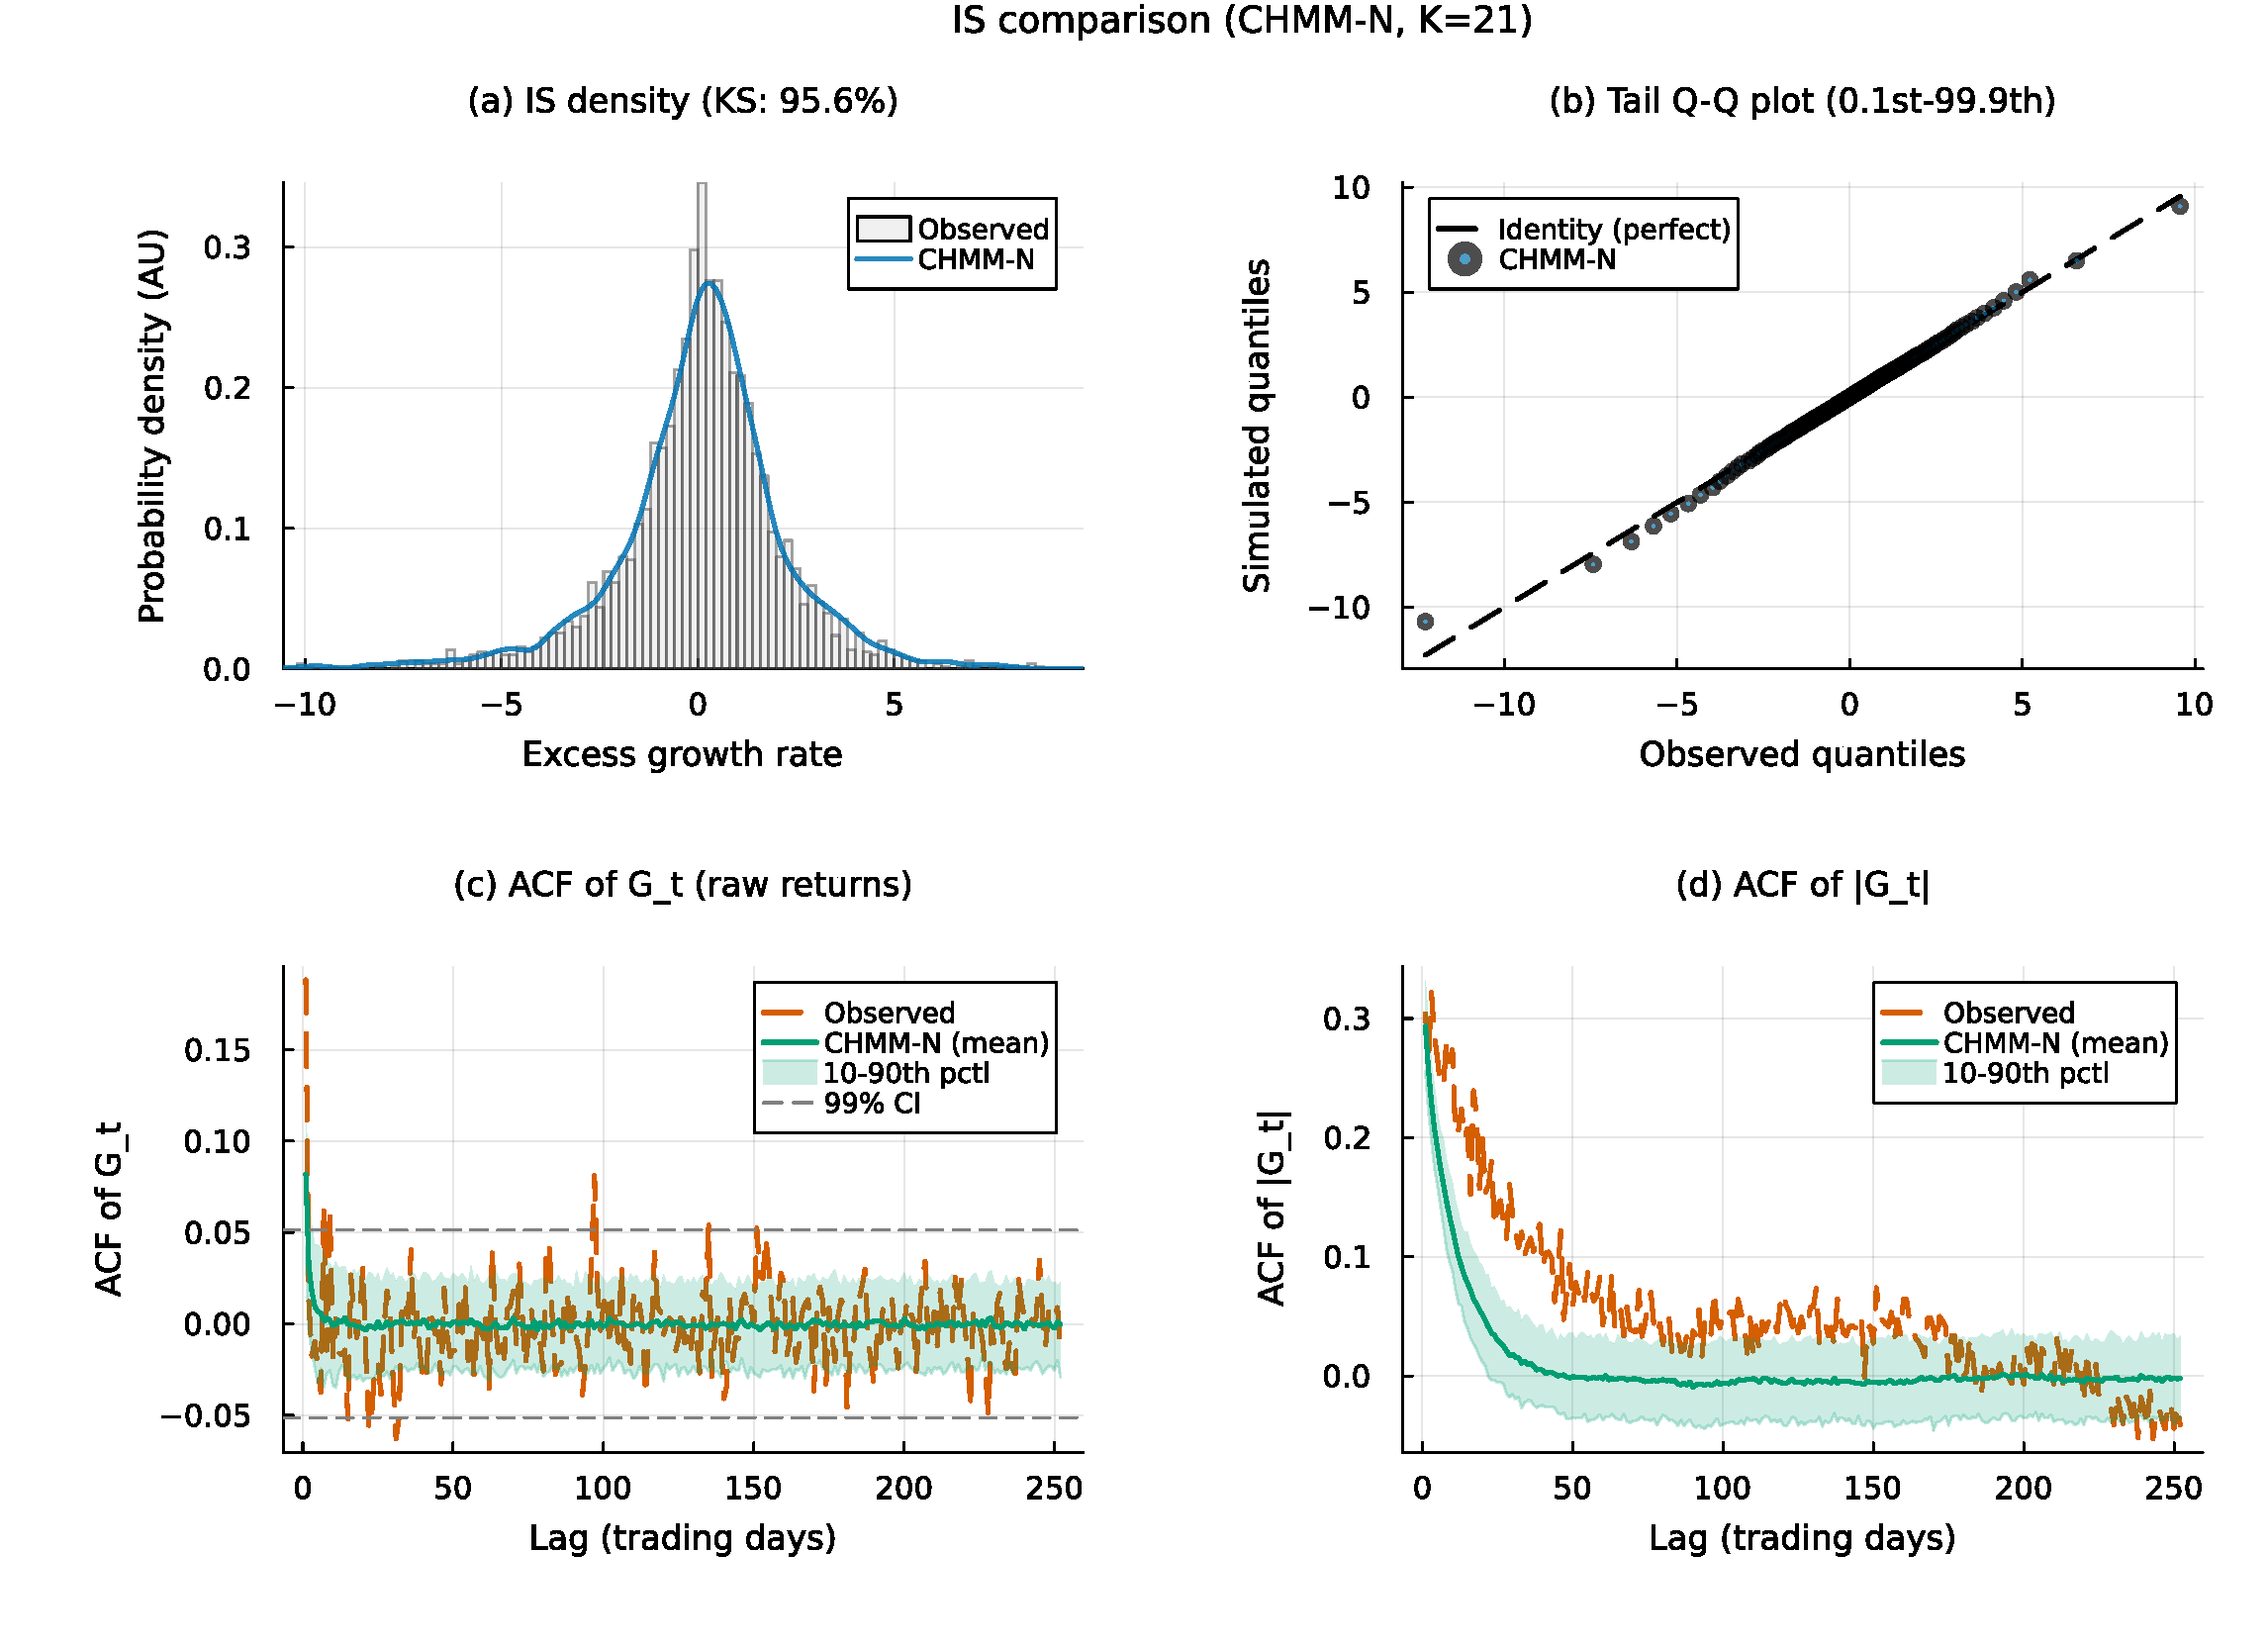
\includegraphics[width=\textwidth]{figs/Fig-3-IS-Comparison-K21.pdf}
\caption{IS SPY CHMM-N comparison at $K = 21$ (Pipeline~A, 1{,}000 simulated paths; panels as in Figure~\ref{fig:is_comparison}).}
\label{fig:k_sweep_is_k21}
\end{figure}

\subsubsection{OoS Validation at Non-Selected State Resolutions}

Figures~\ref{fig:k_sweep_panels_oos}--\ref{fig:k_sweep_oos_k21} show the OoS validation panels for $K \in \{3, 6, 12, 21\}$.
KS pass rates remain above 91\% at all resolutions; the $K = 18$ panel is reproduced in Figure~\ref{fig:oos_validation} of the main text.
As with the IS panels, $K = 9$ and $K = 15$ are omitted; numerical OoS KS pass rates are in Table~\ref{tab:sensitivity}.

\begin{figure}[H]
\centering
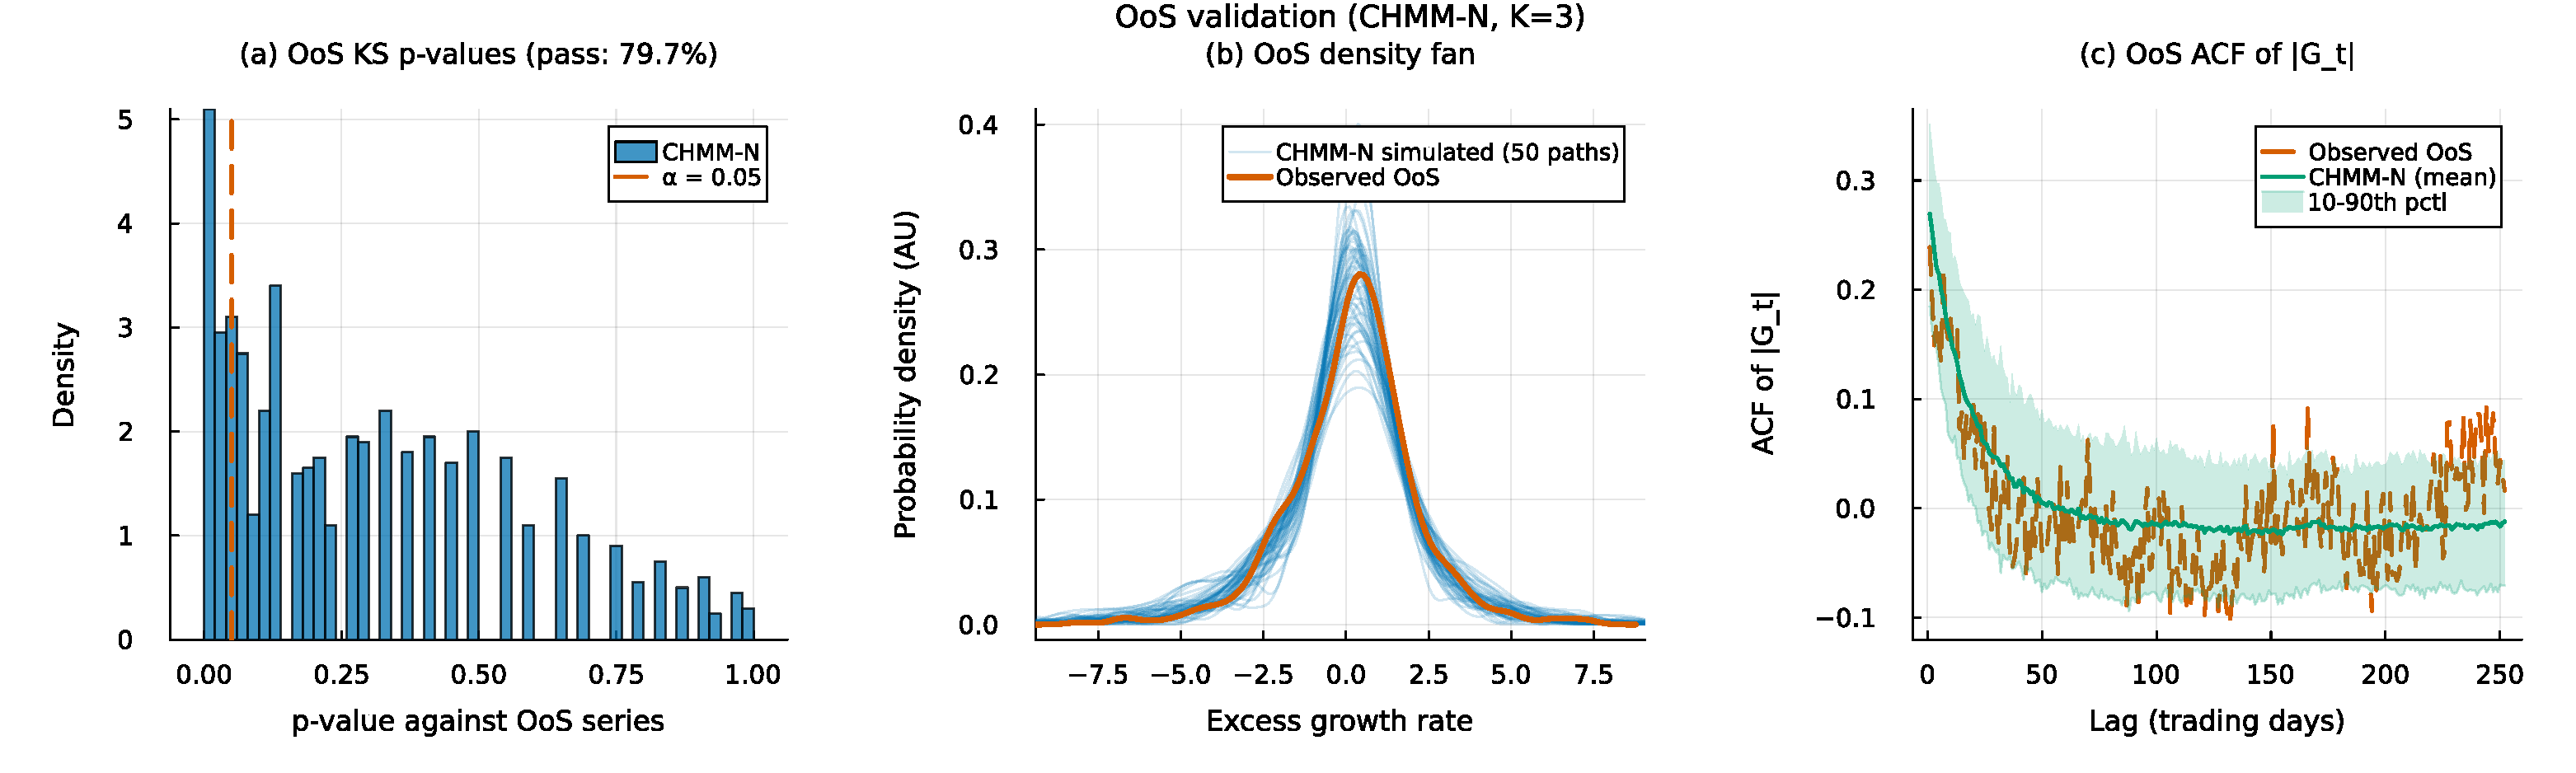
\includegraphics[width=\textwidth]{figs/Fig-4-OoS-Validation-K3.pdf}
\caption{OoS SPY CHMM-N validation at $K = 3$ (Pipeline~A, 1{,}000 simulated paths; panels as in Figure~\ref{fig:oos_validation}). The $K = 18$ counterpart is Figure~\ref{fig:oos_validation} of the main text.}
\label{fig:k_sweep_panels_oos}
\end{figure}

\begin{figure}[H]
\centering
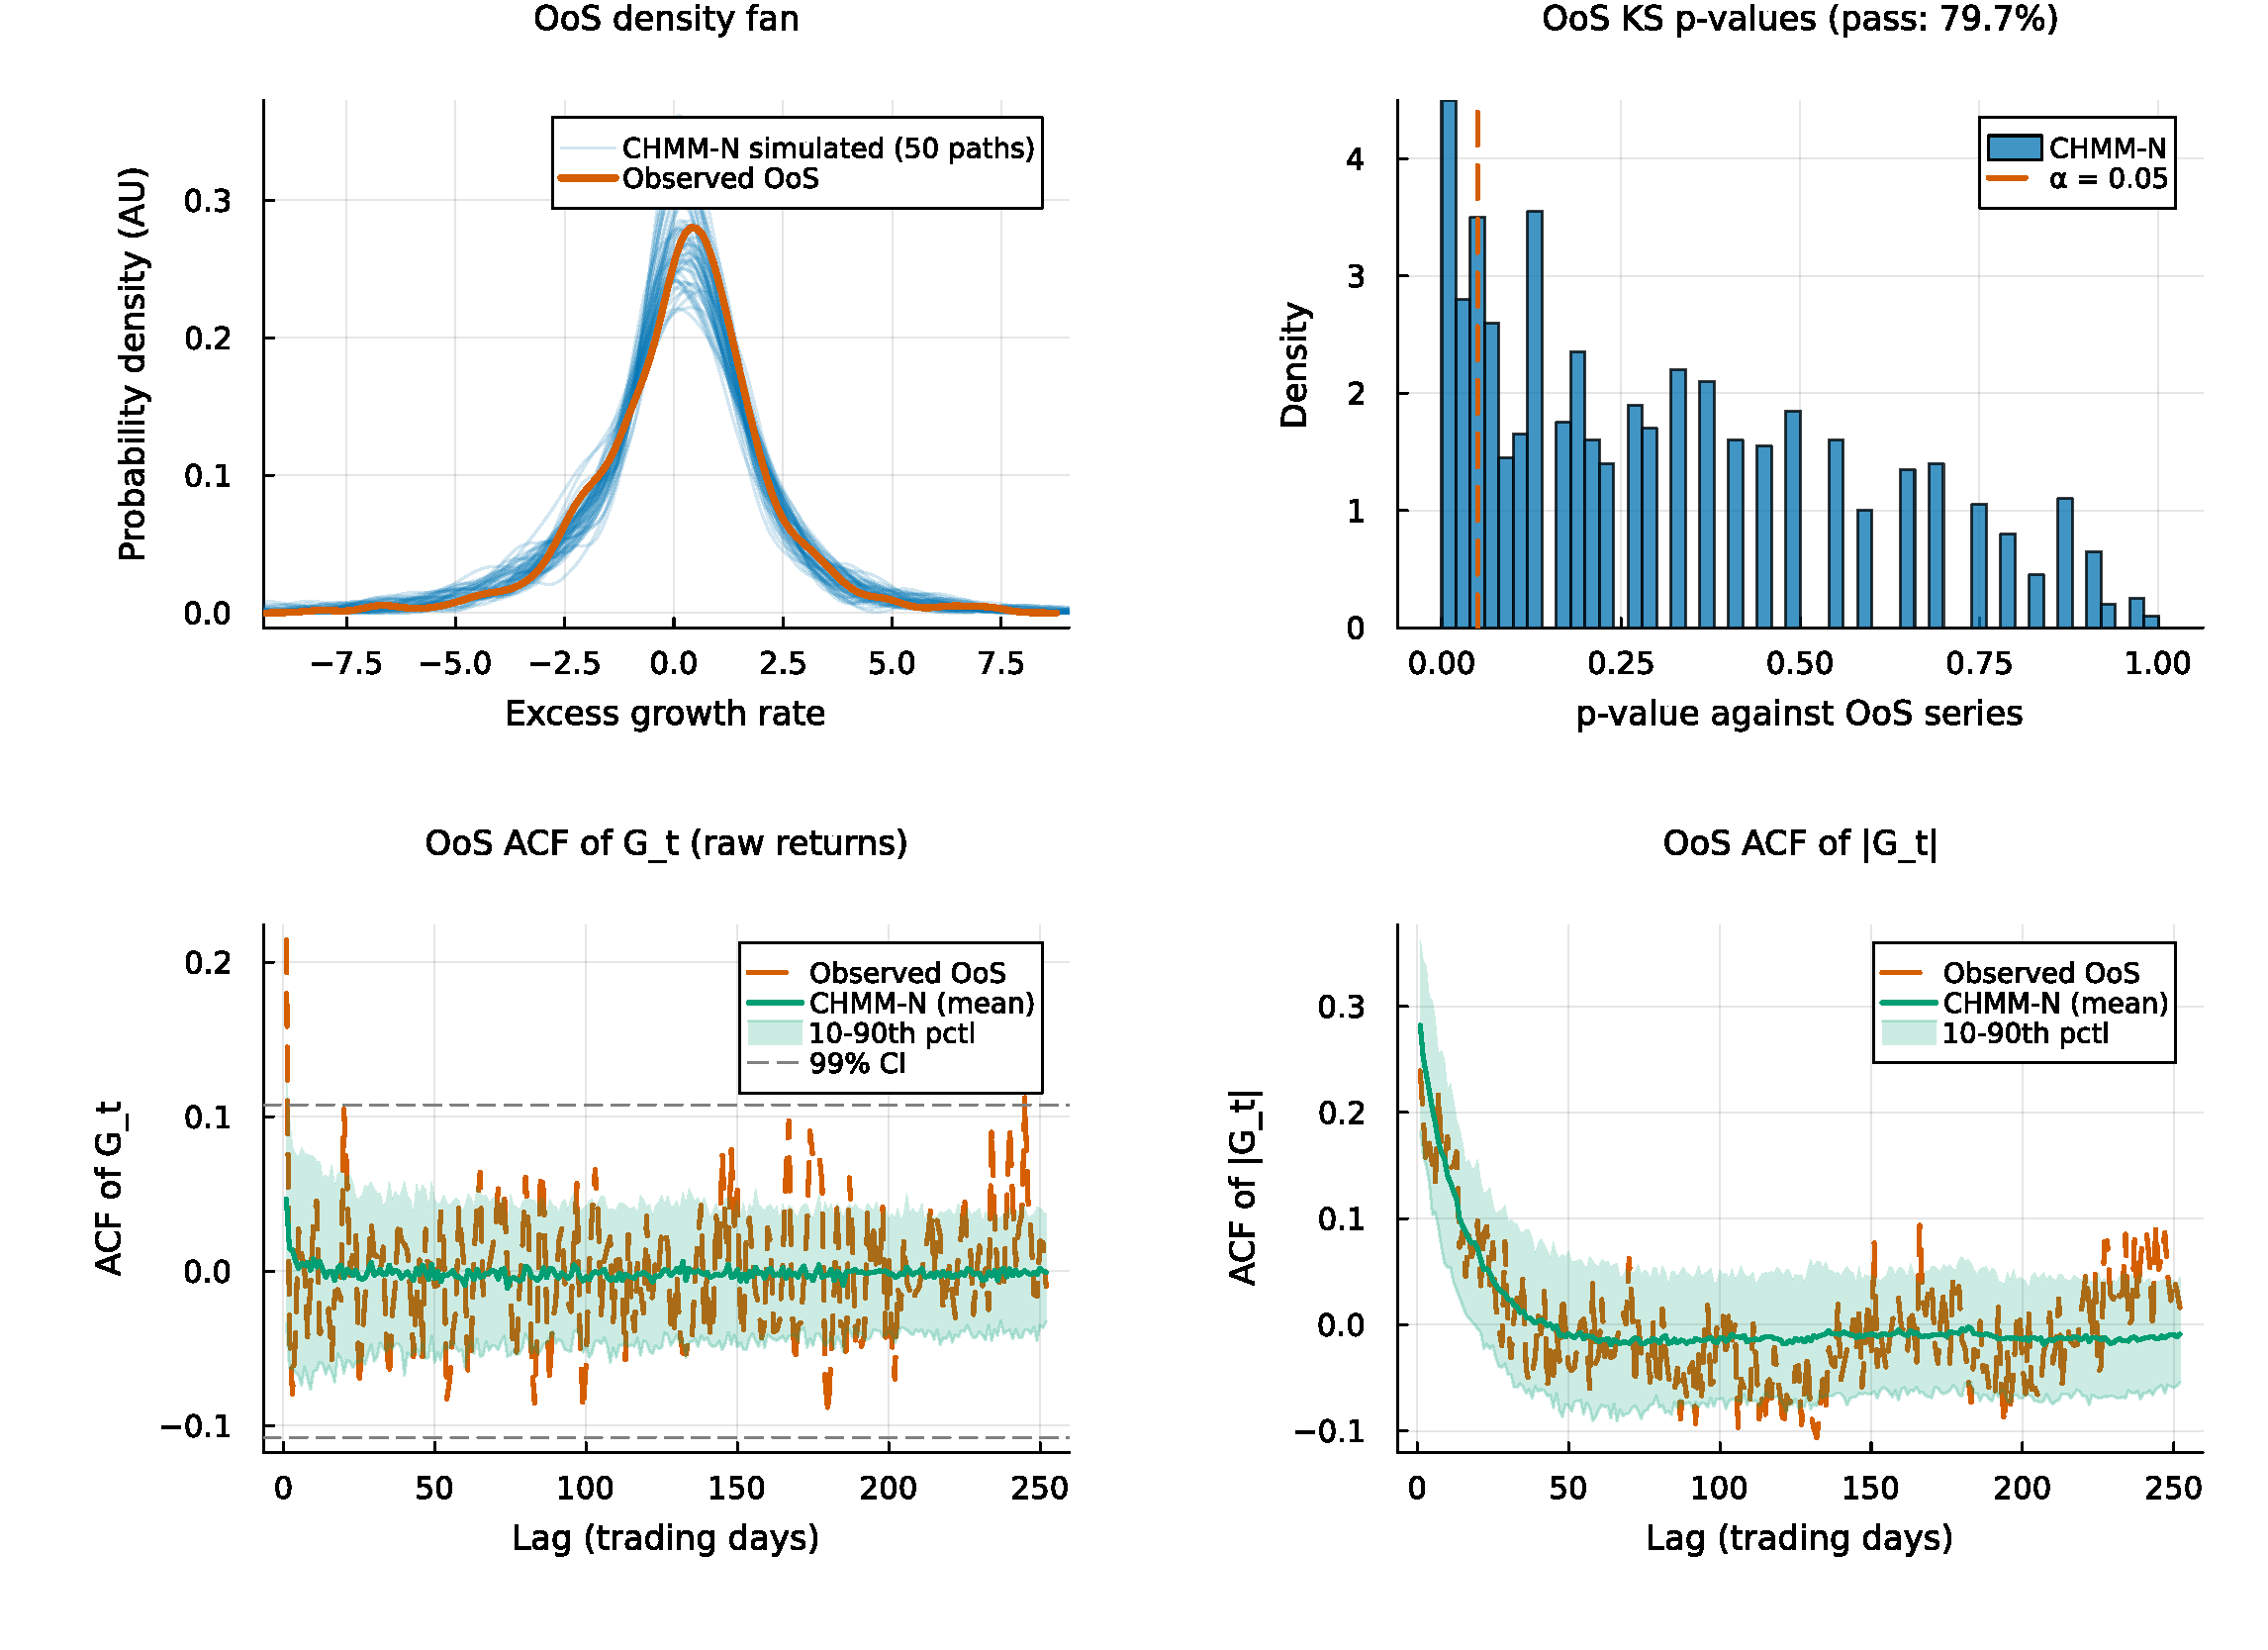
\includegraphics[width=\textwidth]{figs/Fig-4-OoS-Validation-K6.pdf}
\caption{OoS SPY CHMM-N validation at $K = 6$ (Pipeline~A, 1{,}000 simulated paths; panels as in Figure~\ref{fig:oos_validation}).}
\label{fig:k_sweep_oos_k6}
\end{figure}

\begin{figure}[H]
\centering
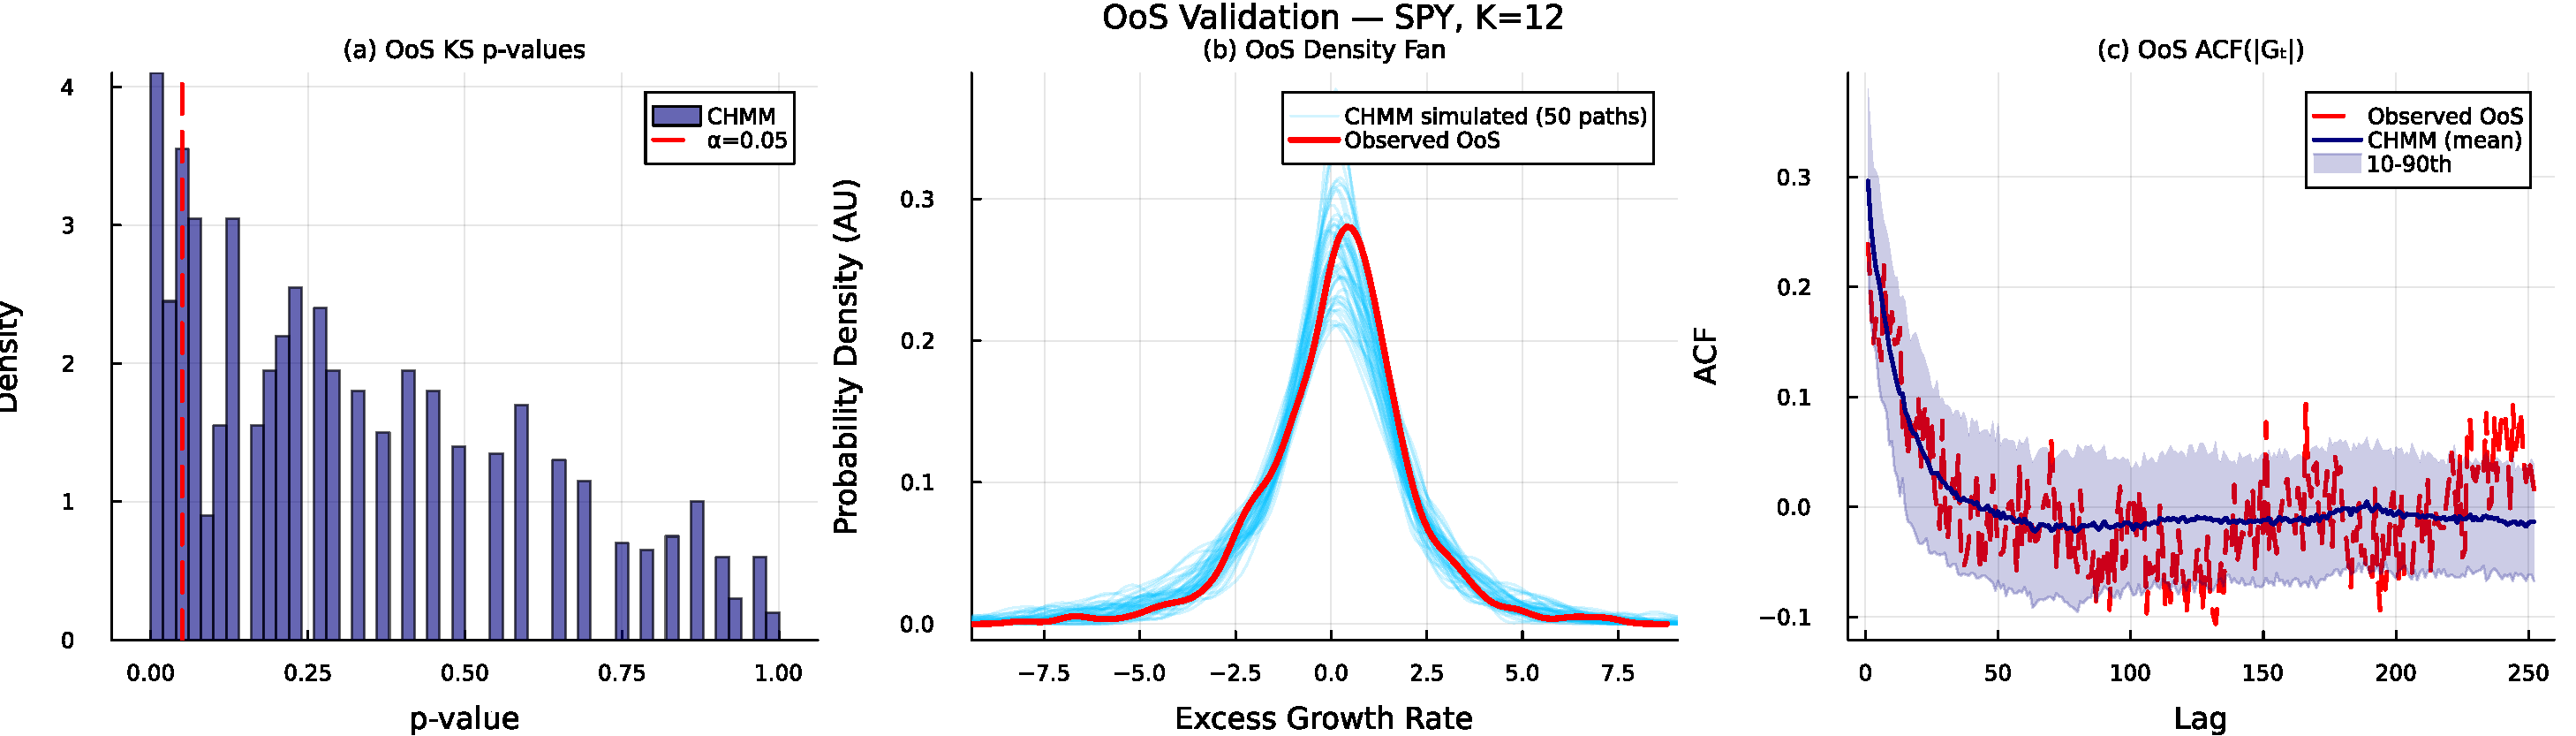
\includegraphics[width=\textwidth]{figs/Fig-4-OoS-Validation-K12.pdf}
\caption{OoS SPY CHMM-N validation at $K = 12$ (Pipeline~A, 1{,}000 simulated paths; panels as in Figure~\ref{fig:oos_validation}).}
\label{fig:k_sweep_oos_k12}
\end{figure}

\begin{figure}[H]
\centering
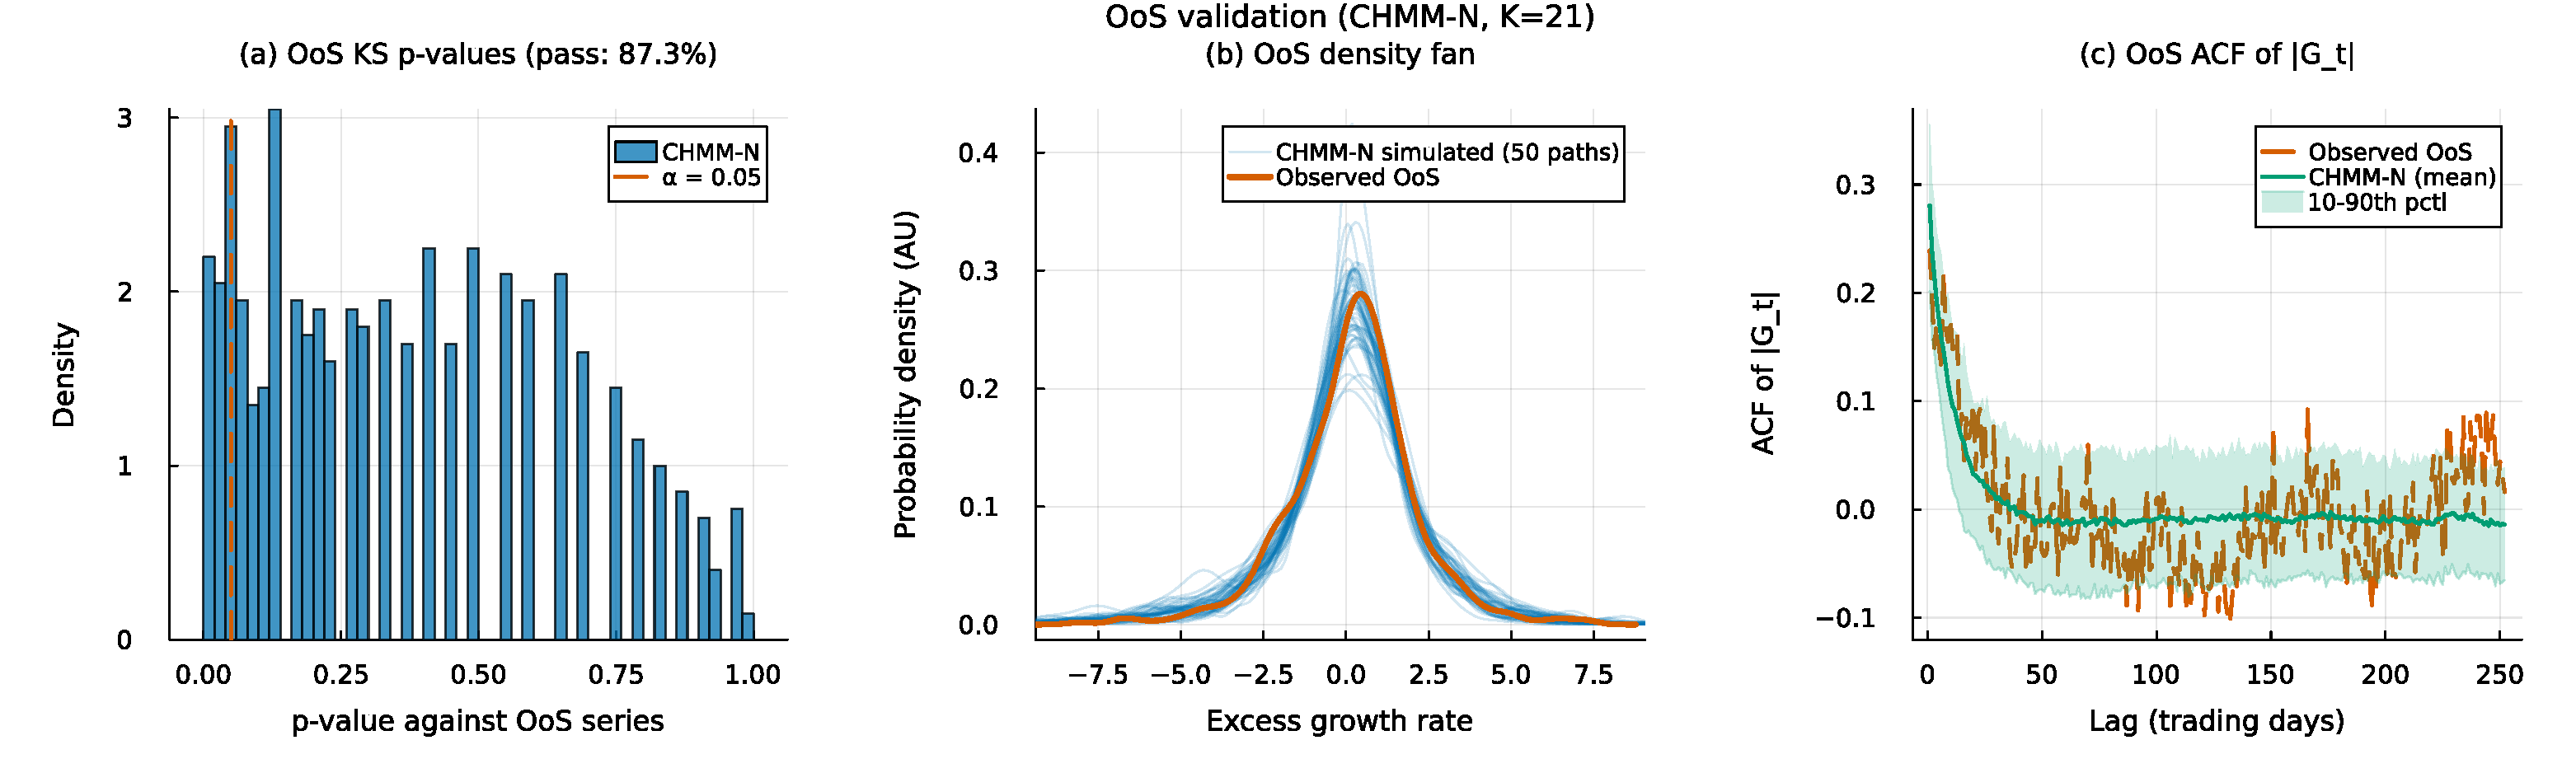
\includegraphics[width=\textwidth]{figs/Fig-4-OoS-Validation-K21.pdf}
\caption{OoS SPY CHMM-N validation at $K = 21$ (Pipeline~A, 1{,}000 simulated paths; panels as in Figure~\ref{fig:oos_validation}).}
\label{fig:k_sweep_oos_k21}
\end{figure}

\subsubsection{\texorpdfstring{Multi-Emission Figures at $K = 18$}{Multi-Emission Figures at K = 18}}
\label{sec:multi_emission_figs}

This appendix reproduces the standard diagnostic suite (emission PDFs, residence times, IS comparison, OoS validation, and convergence) for the two heavy-tailed emission families (CHMM-t and CHMM-L) at the selected state resolution $K = 18$; transition matrices and stationary distributions are discussed in prose only below, since they are visually indistinguishable across families at $K = 18$.
The Gaussian counterparts are already shown as Figures~\ref{fig:is_comparison} and~\ref{fig:oos_validation} in the main text and as Figure~\ref{fig:convergence_all} above in this appendix.
The figures confirm that the shared forward--backward scaffold produces internally-similar regime structure across the three families: the near-diagonal transition band, the $K$-component dense emission cover, the longer central-state residence times, and the monotone log-likelihood convergence are features of the CHMM framework and not of the Gaussian component specifically.

\paragraph{Emission PDFs.}
Figure~\ref{fig:emissions_families} compares the learned $K = 18$ emissions for the three families.
The CHMM-t panel's per-state $\nu_k$ allocation is visible in the narrower modes of certain tail states; the CHMM-L panel's Laplace components have sharper peaks and slower exponential tail decay than the Gaussians.

\begin{figure}[H]
\centering
\begin{subfigure}[b]{0.32\textwidth}
    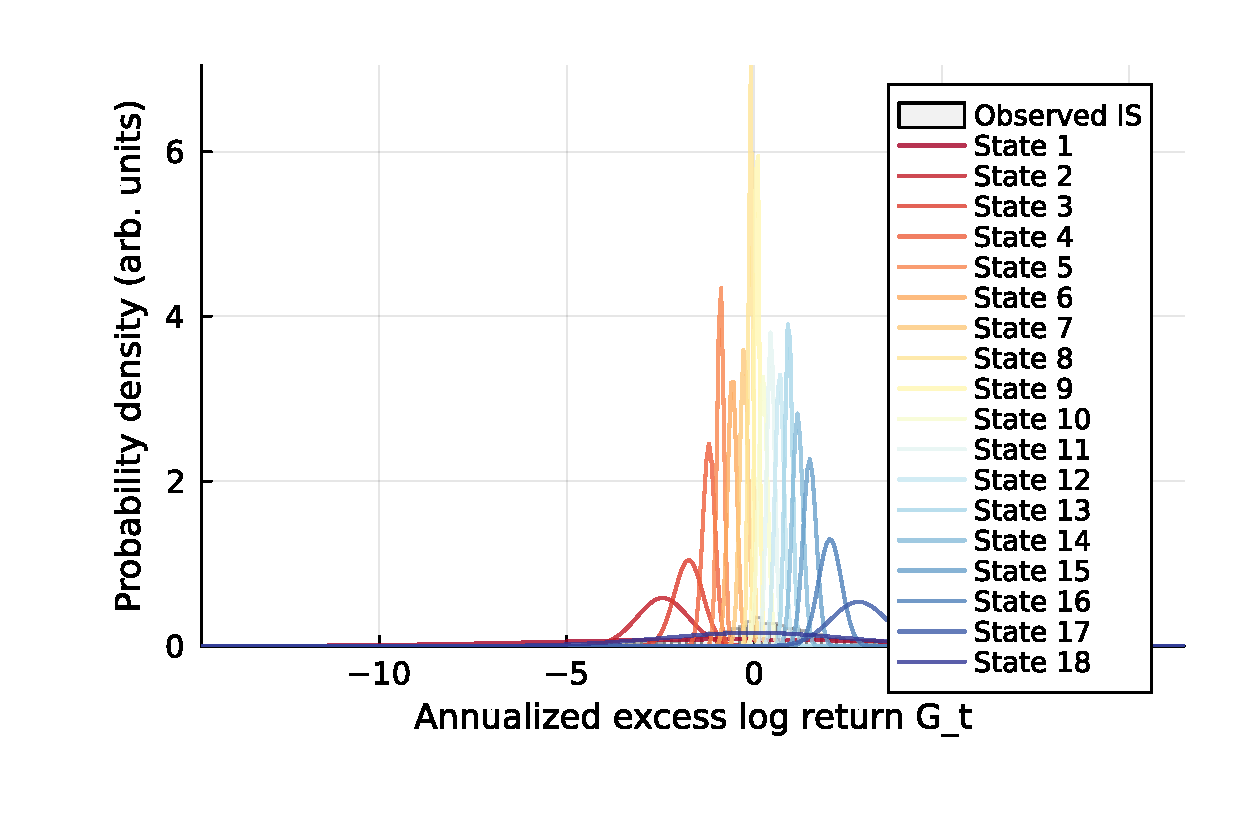
\includegraphics[width=\textwidth]{figs/Fig-Emission-PDFs-K18-N.pdf}
    \caption{CHMM-N (Gaussian)}
\end{subfigure}
\hfill
\begin{subfigure}[b]{0.32\textwidth}
    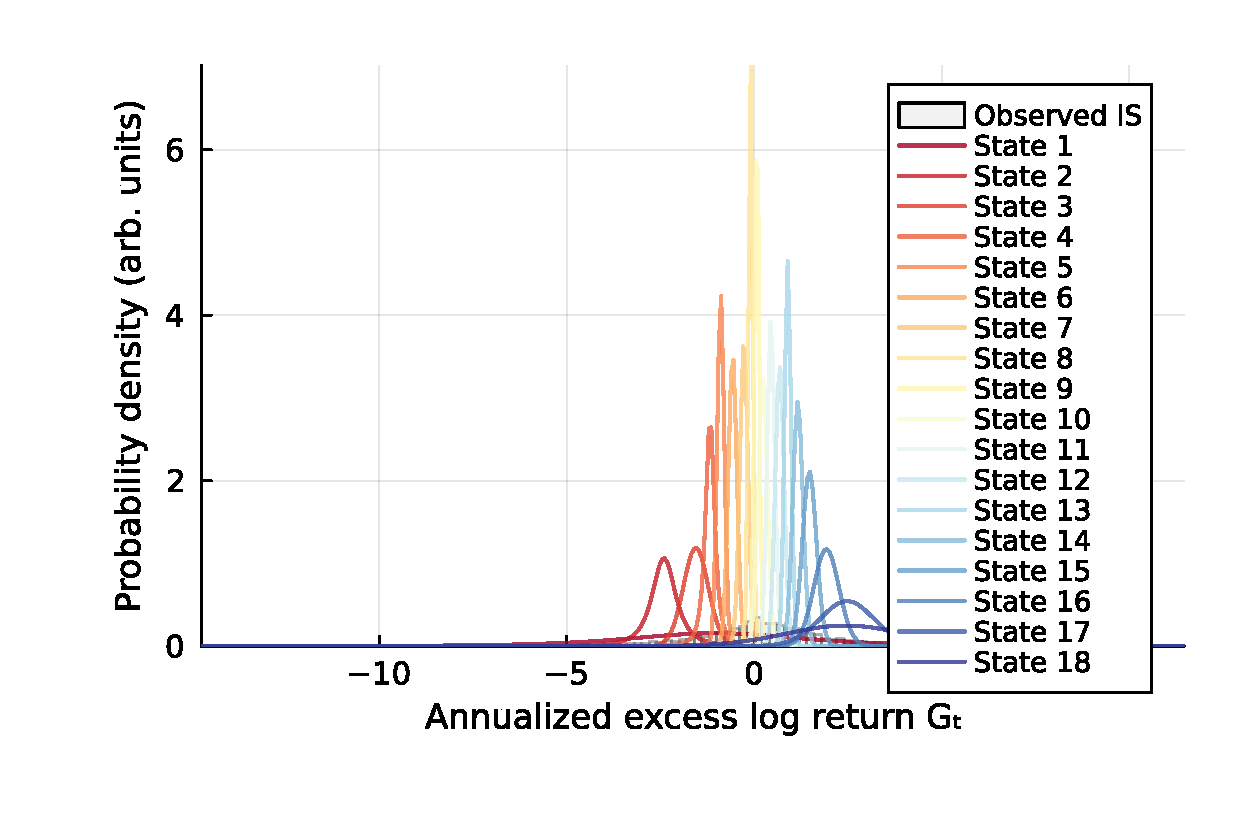
\includegraphics[width=\textwidth]{figs/Fig-Emission-PDFs-K18-t.pdf}
    \caption{CHMM-t (Student-t)}
\end{subfigure}
\hfill
\begin{subfigure}[b]{0.32\textwidth}
    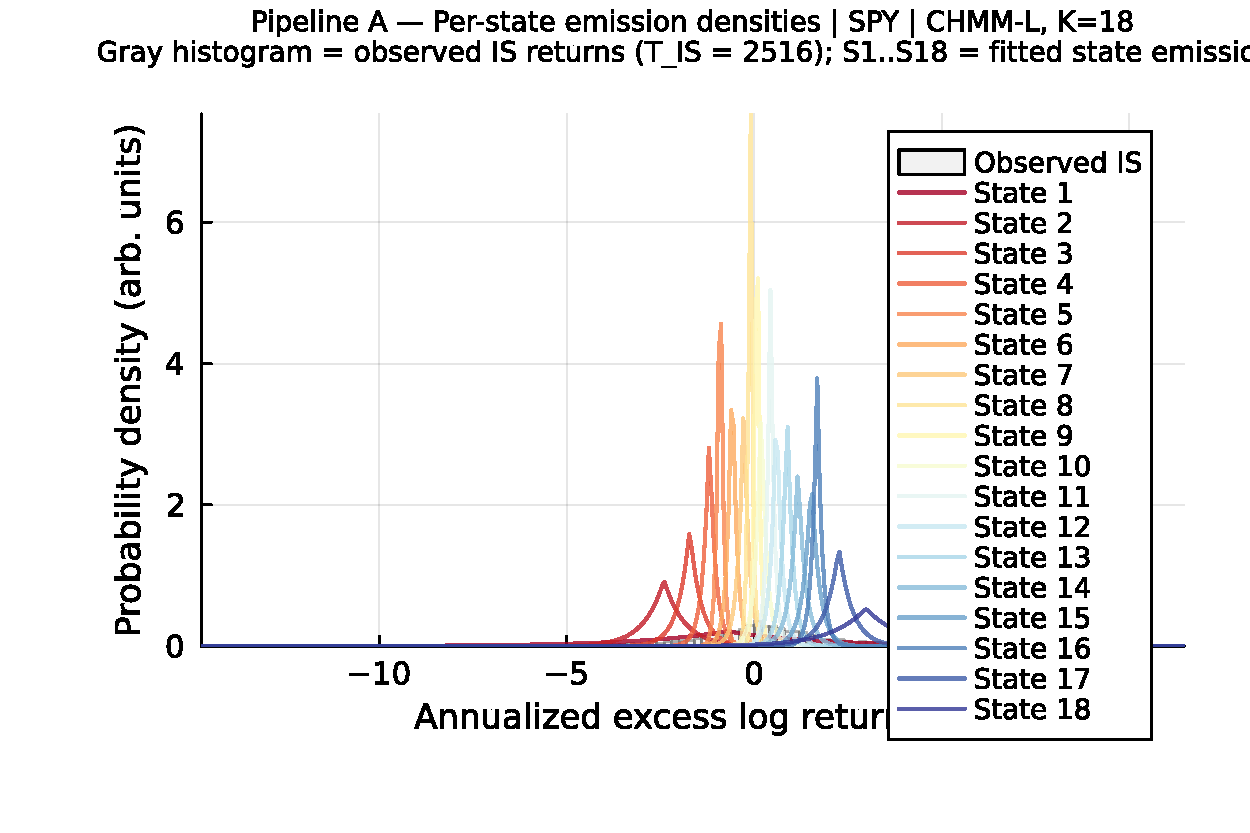
\includegraphics[width=\textwidth]{figs/Fig-Emission-PDFs-K18-L.pdf}
    \caption{CHMM-L (Laplace)}
\end{subfigure}
\caption{Learned emission distributions at $K = 18$ across the three emission families (CHMM-N Gaussian, CHMM-t Student-t with per-state $\nu_k$, CHMM-L Laplace), overlaid on the observed SPY IS return histogram (Pipeline~A). Heavier-tailed emission families (t, L) give individual components more tail mass, which is what closes the kurtosis gap of the Gaussian CHMM.}
\label{fig:emissions_families}
\end{figure}

\paragraph{Transition matrices and stationary distributions.}
The $K = 18$ transition matrices and stationary distributions learned under CHMM-t and CHMM-L are visually indistinguishable from their CHMM-N counterparts: the near-diagonal band, the magnitude of self-transition probabilities, and the mass concentration at central states are features of the regime structure, not the emission family. This is consistent with the ACF-MAE being stable across the family axis (Table~\ref{tab:sensitivity_multi}). The per-family residence times $\tau_k = 1/(1 - T_{kk})$, which magnify small differences in the self-transition probabilities each family recovers, are compared in Figure~\ref{fig:residence_families}.

\begin{figure}[H]
\centering
\begin{subfigure}[b]{0.32\textwidth}
    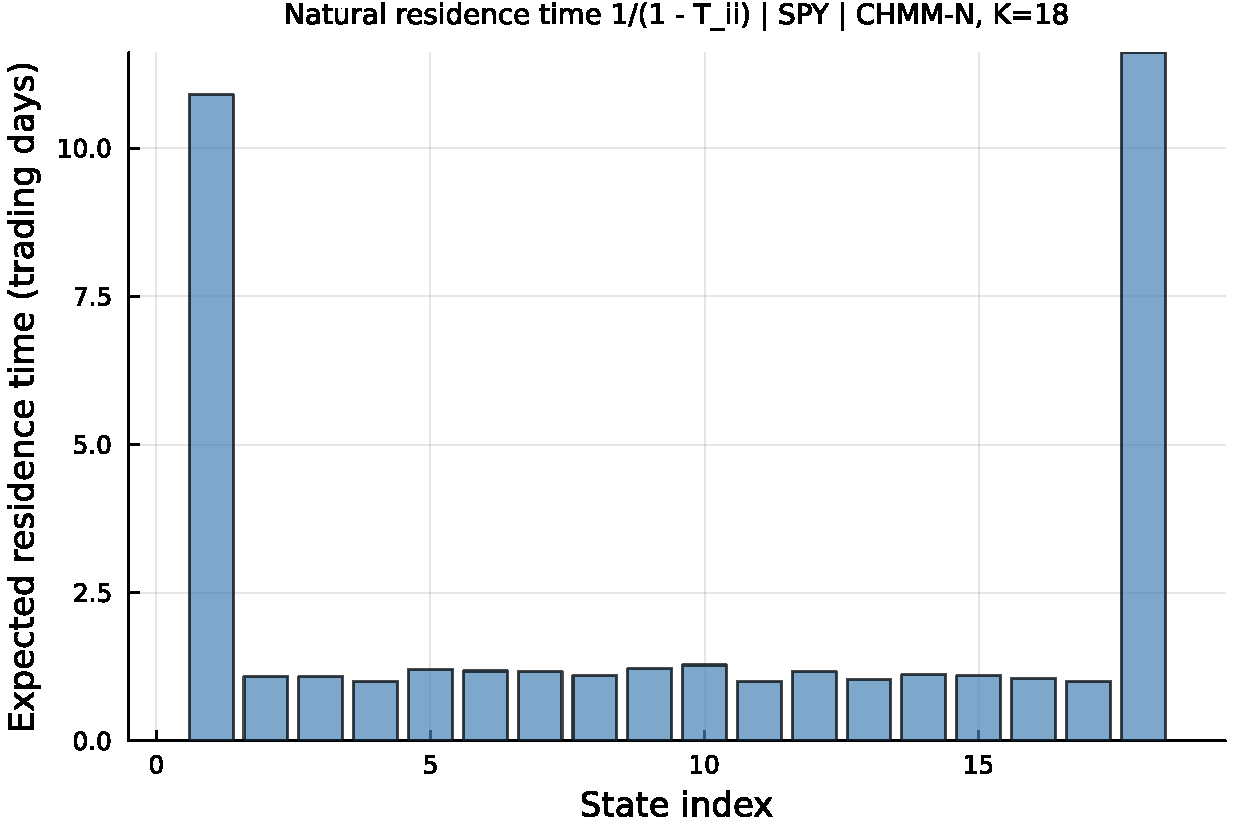
\includegraphics[width=\textwidth]{figs/Fig-Residence-Times-K18-N.pdf}
    \caption{CHMM-N}
\end{subfigure}
\hfill
\begin{subfigure}[b]{0.32\textwidth}
    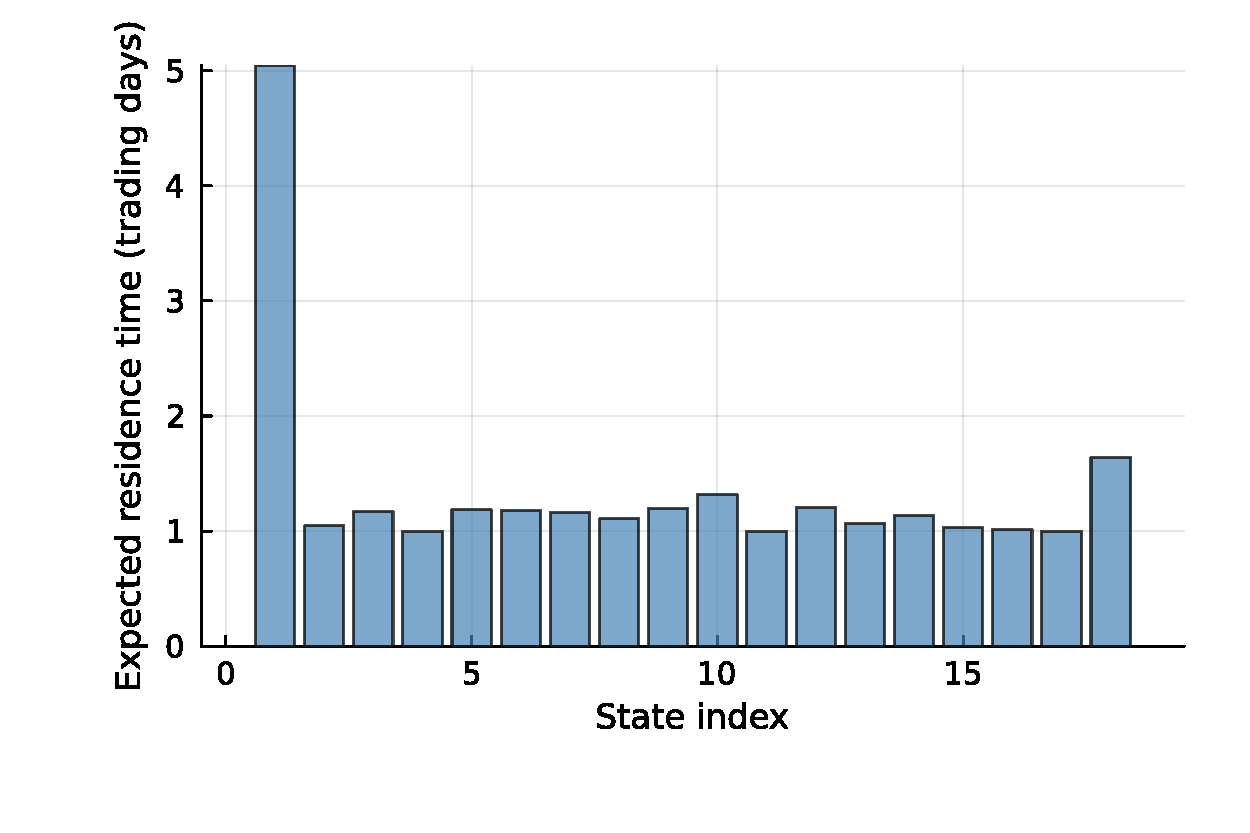
\includegraphics[width=\textwidth]{figs/Fig-Residence-Times-K18-t.pdf}
    \caption{CHMM-t}
\end{subfigure}
\hfill
\begin{subfigure}[b]{0.32\textwidth}
    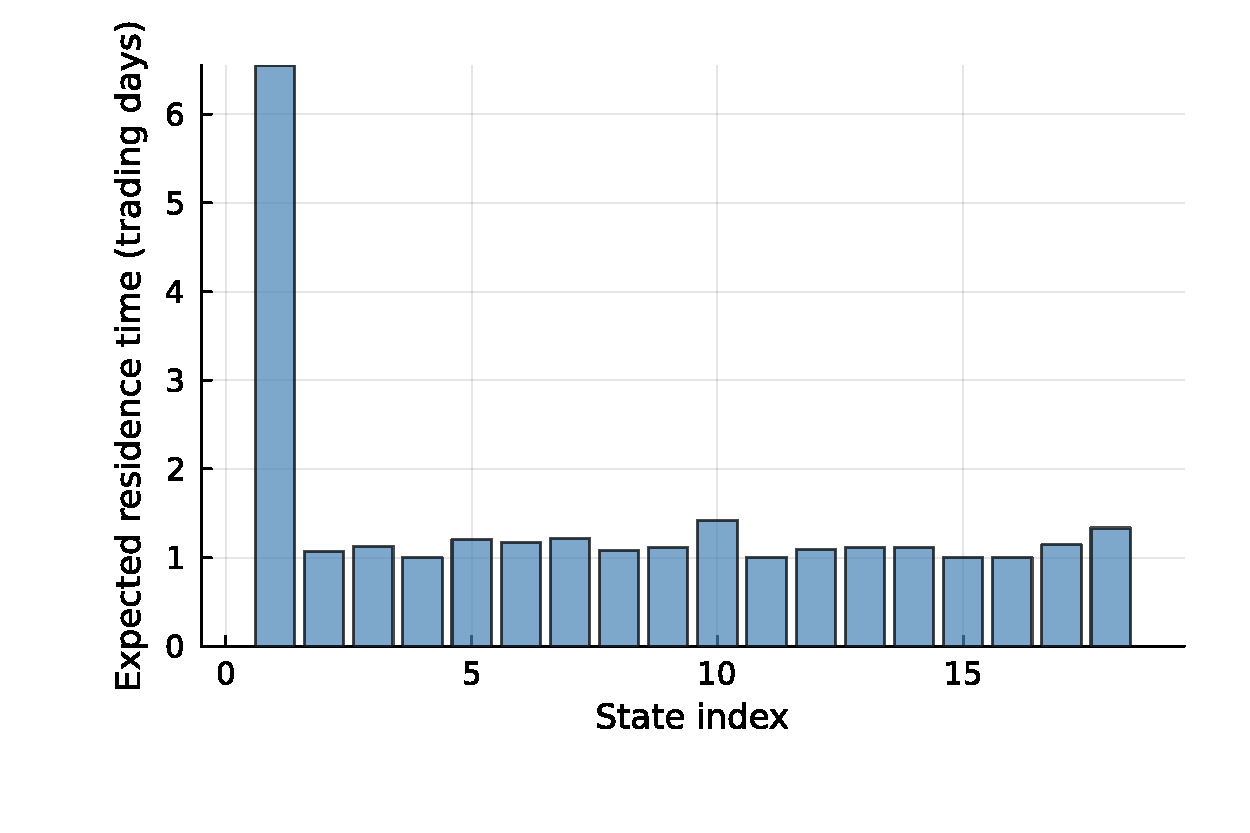
\includegraphics[width=\textwidth]{figs/Fig-Residence-Times-K18-L.pdf}
    \caption{CHMM-L}
\end{subfigure}
\caption{Natural residence times $\tau_k = 1/(1 - T_{kk})$ at $K = 18$ for the SPY IS fit (Pipeline~A) across the three emission families (CHMM-N Gaussian, CHMM-t Student-t, CHMM-L Laplace).}
\label{fig:residence_families}
\end{figure}

\paragraph{IS comparison.}
Figures~\ref{fig:is_families}--\ref{fig:is_families_L} reproduce the three-panel IS comparison (density, ACF of $|G_t|$, tail Q-Q) at $K = 18$ for the two heavy-tailed families; the CHMM-N panel is Figure~\ref{fig:is_comparison} in the main text.

\begin{figure}[H]
\centering
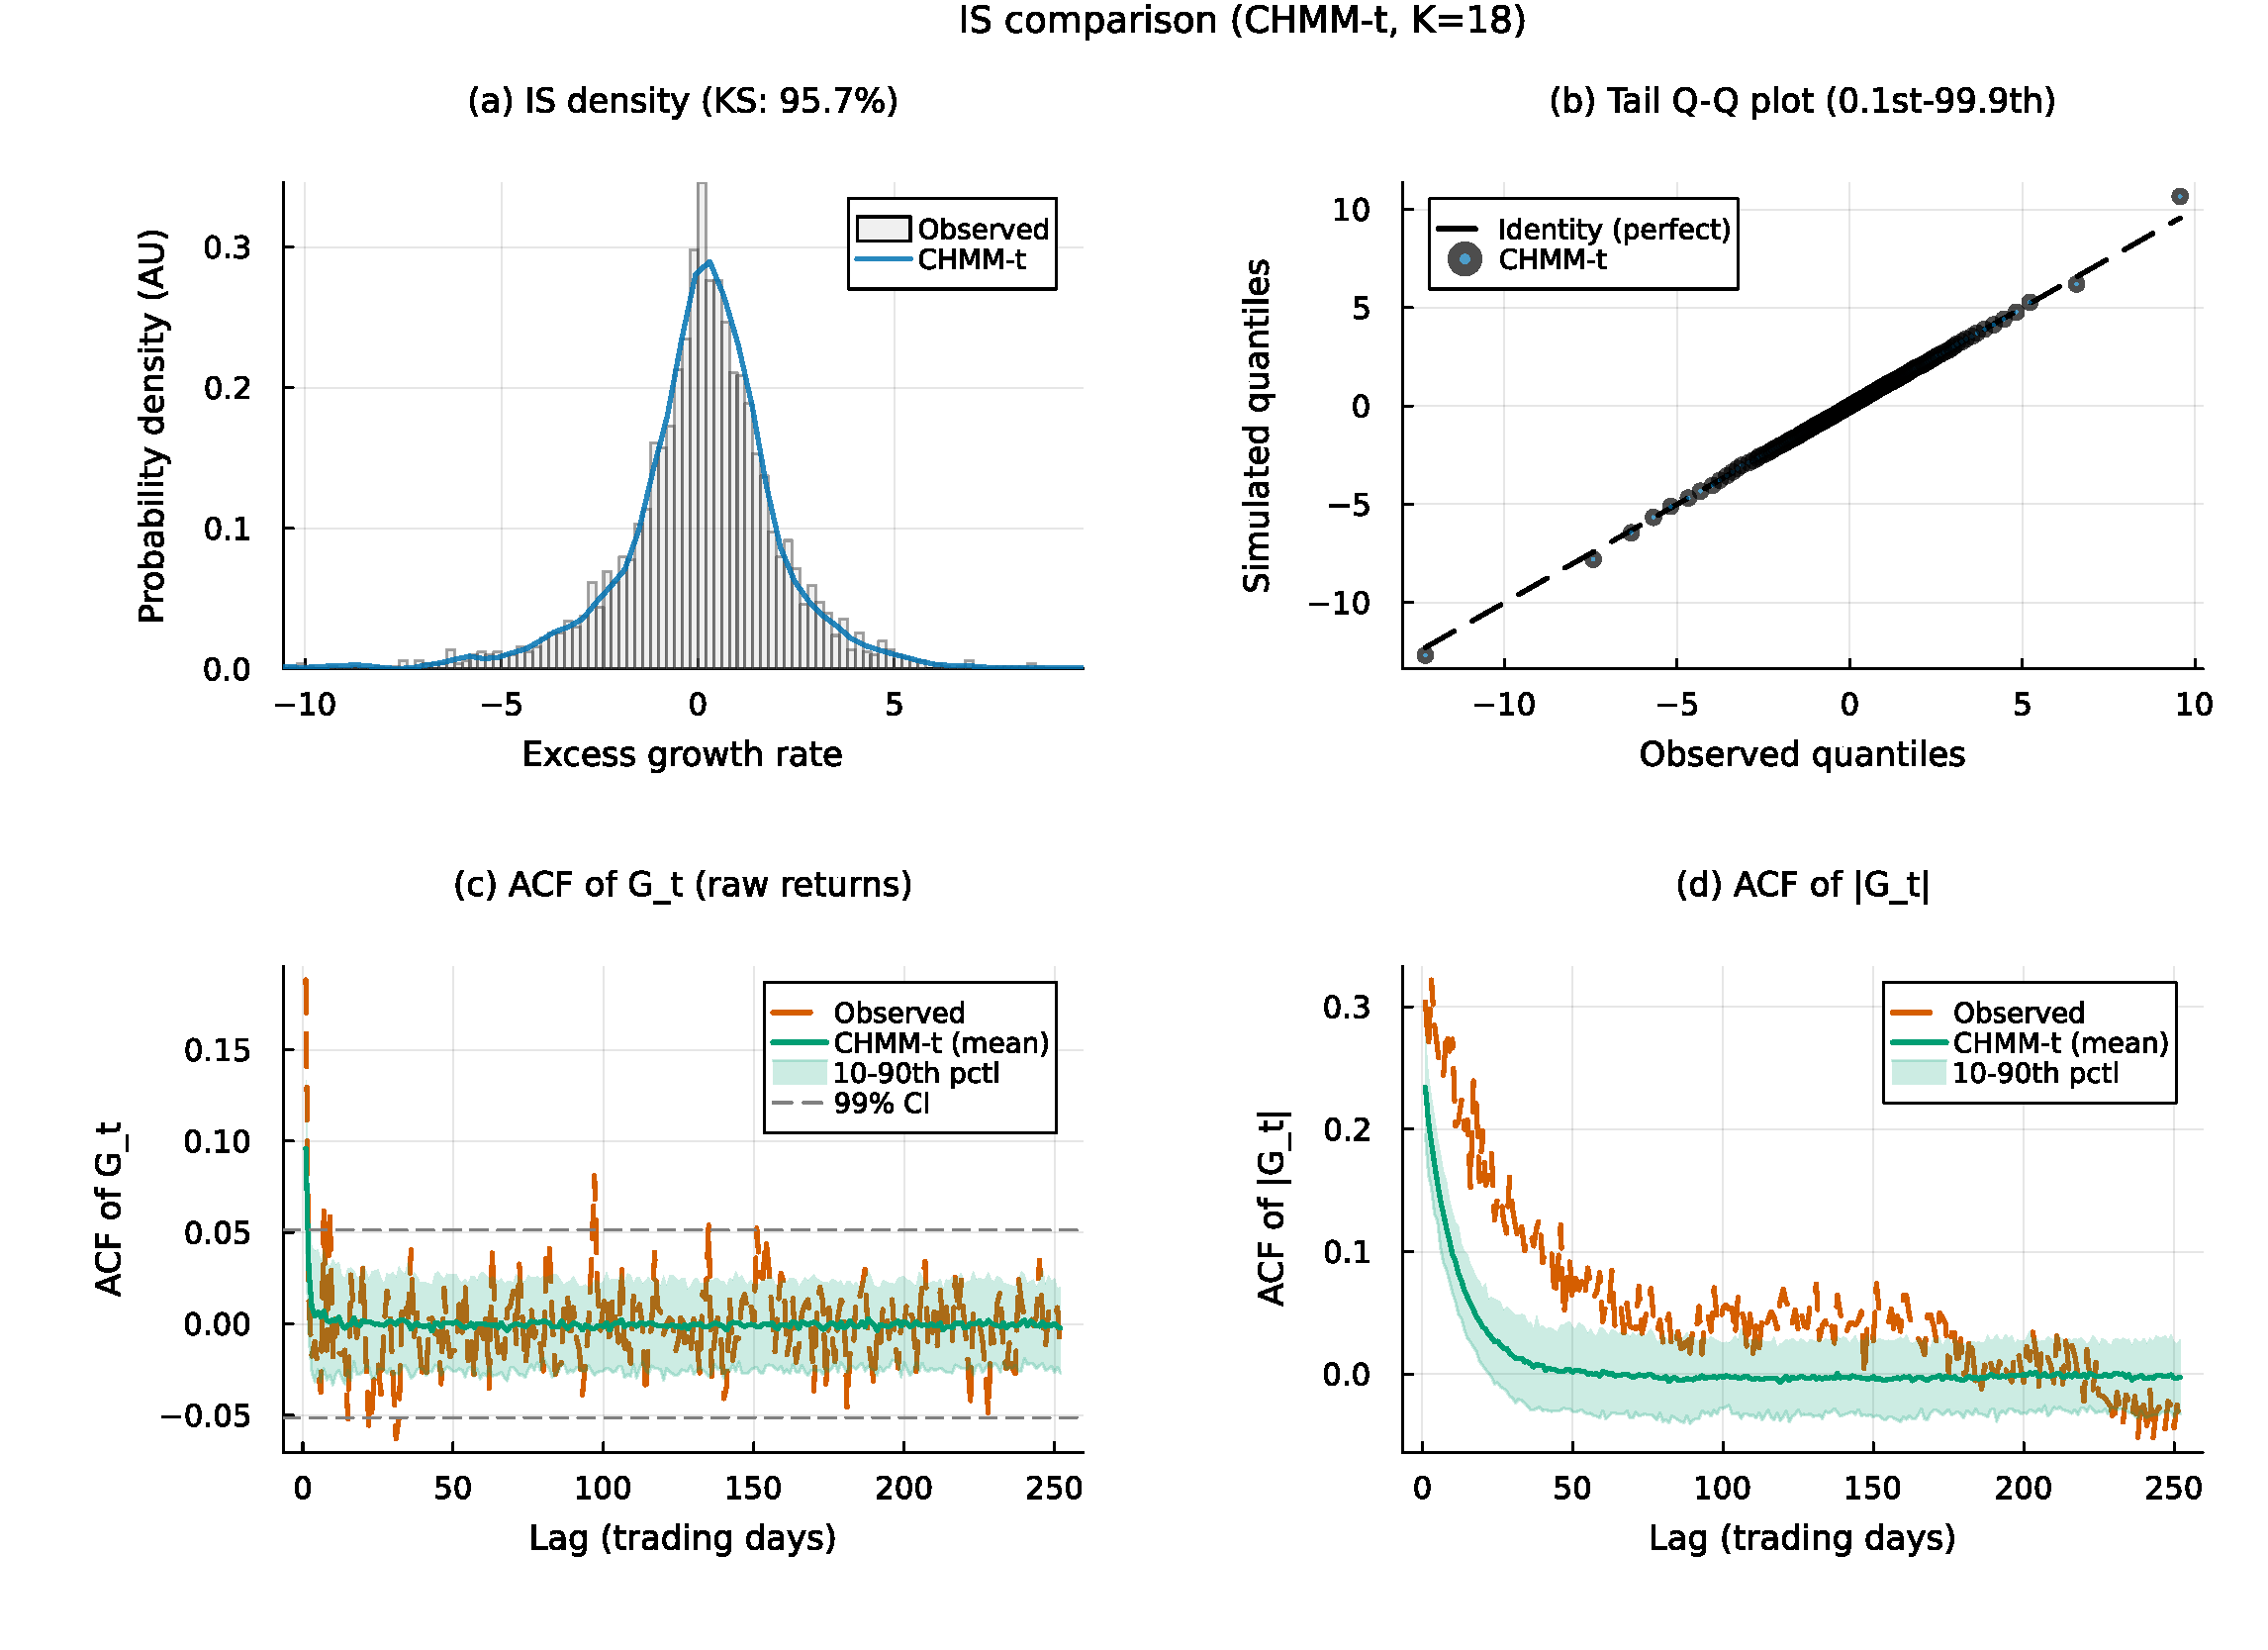
\includegraphics[width=\textwidth]{figs/Fig-3-IS-Comparison-K18-t.pdf}
\caption{IS SPY model comparison at $K = 18$ for CHMM-t Student-t emissions (Pipeline~A, 1{,}000 simulated paths). Panels show (a) marginal density with KS pass rate, (b) ACF of $|G_t|$, and (c) tail Q-Q plot. The CHMM-N counterpart is Figure~\ref{fig:is_comparison}; the CHMM-L counterpart is Figure~\ref{fig:is_families_L}.}
\label{fig:is_families}
\end{figure}

\begin{figure}[H]
\centering
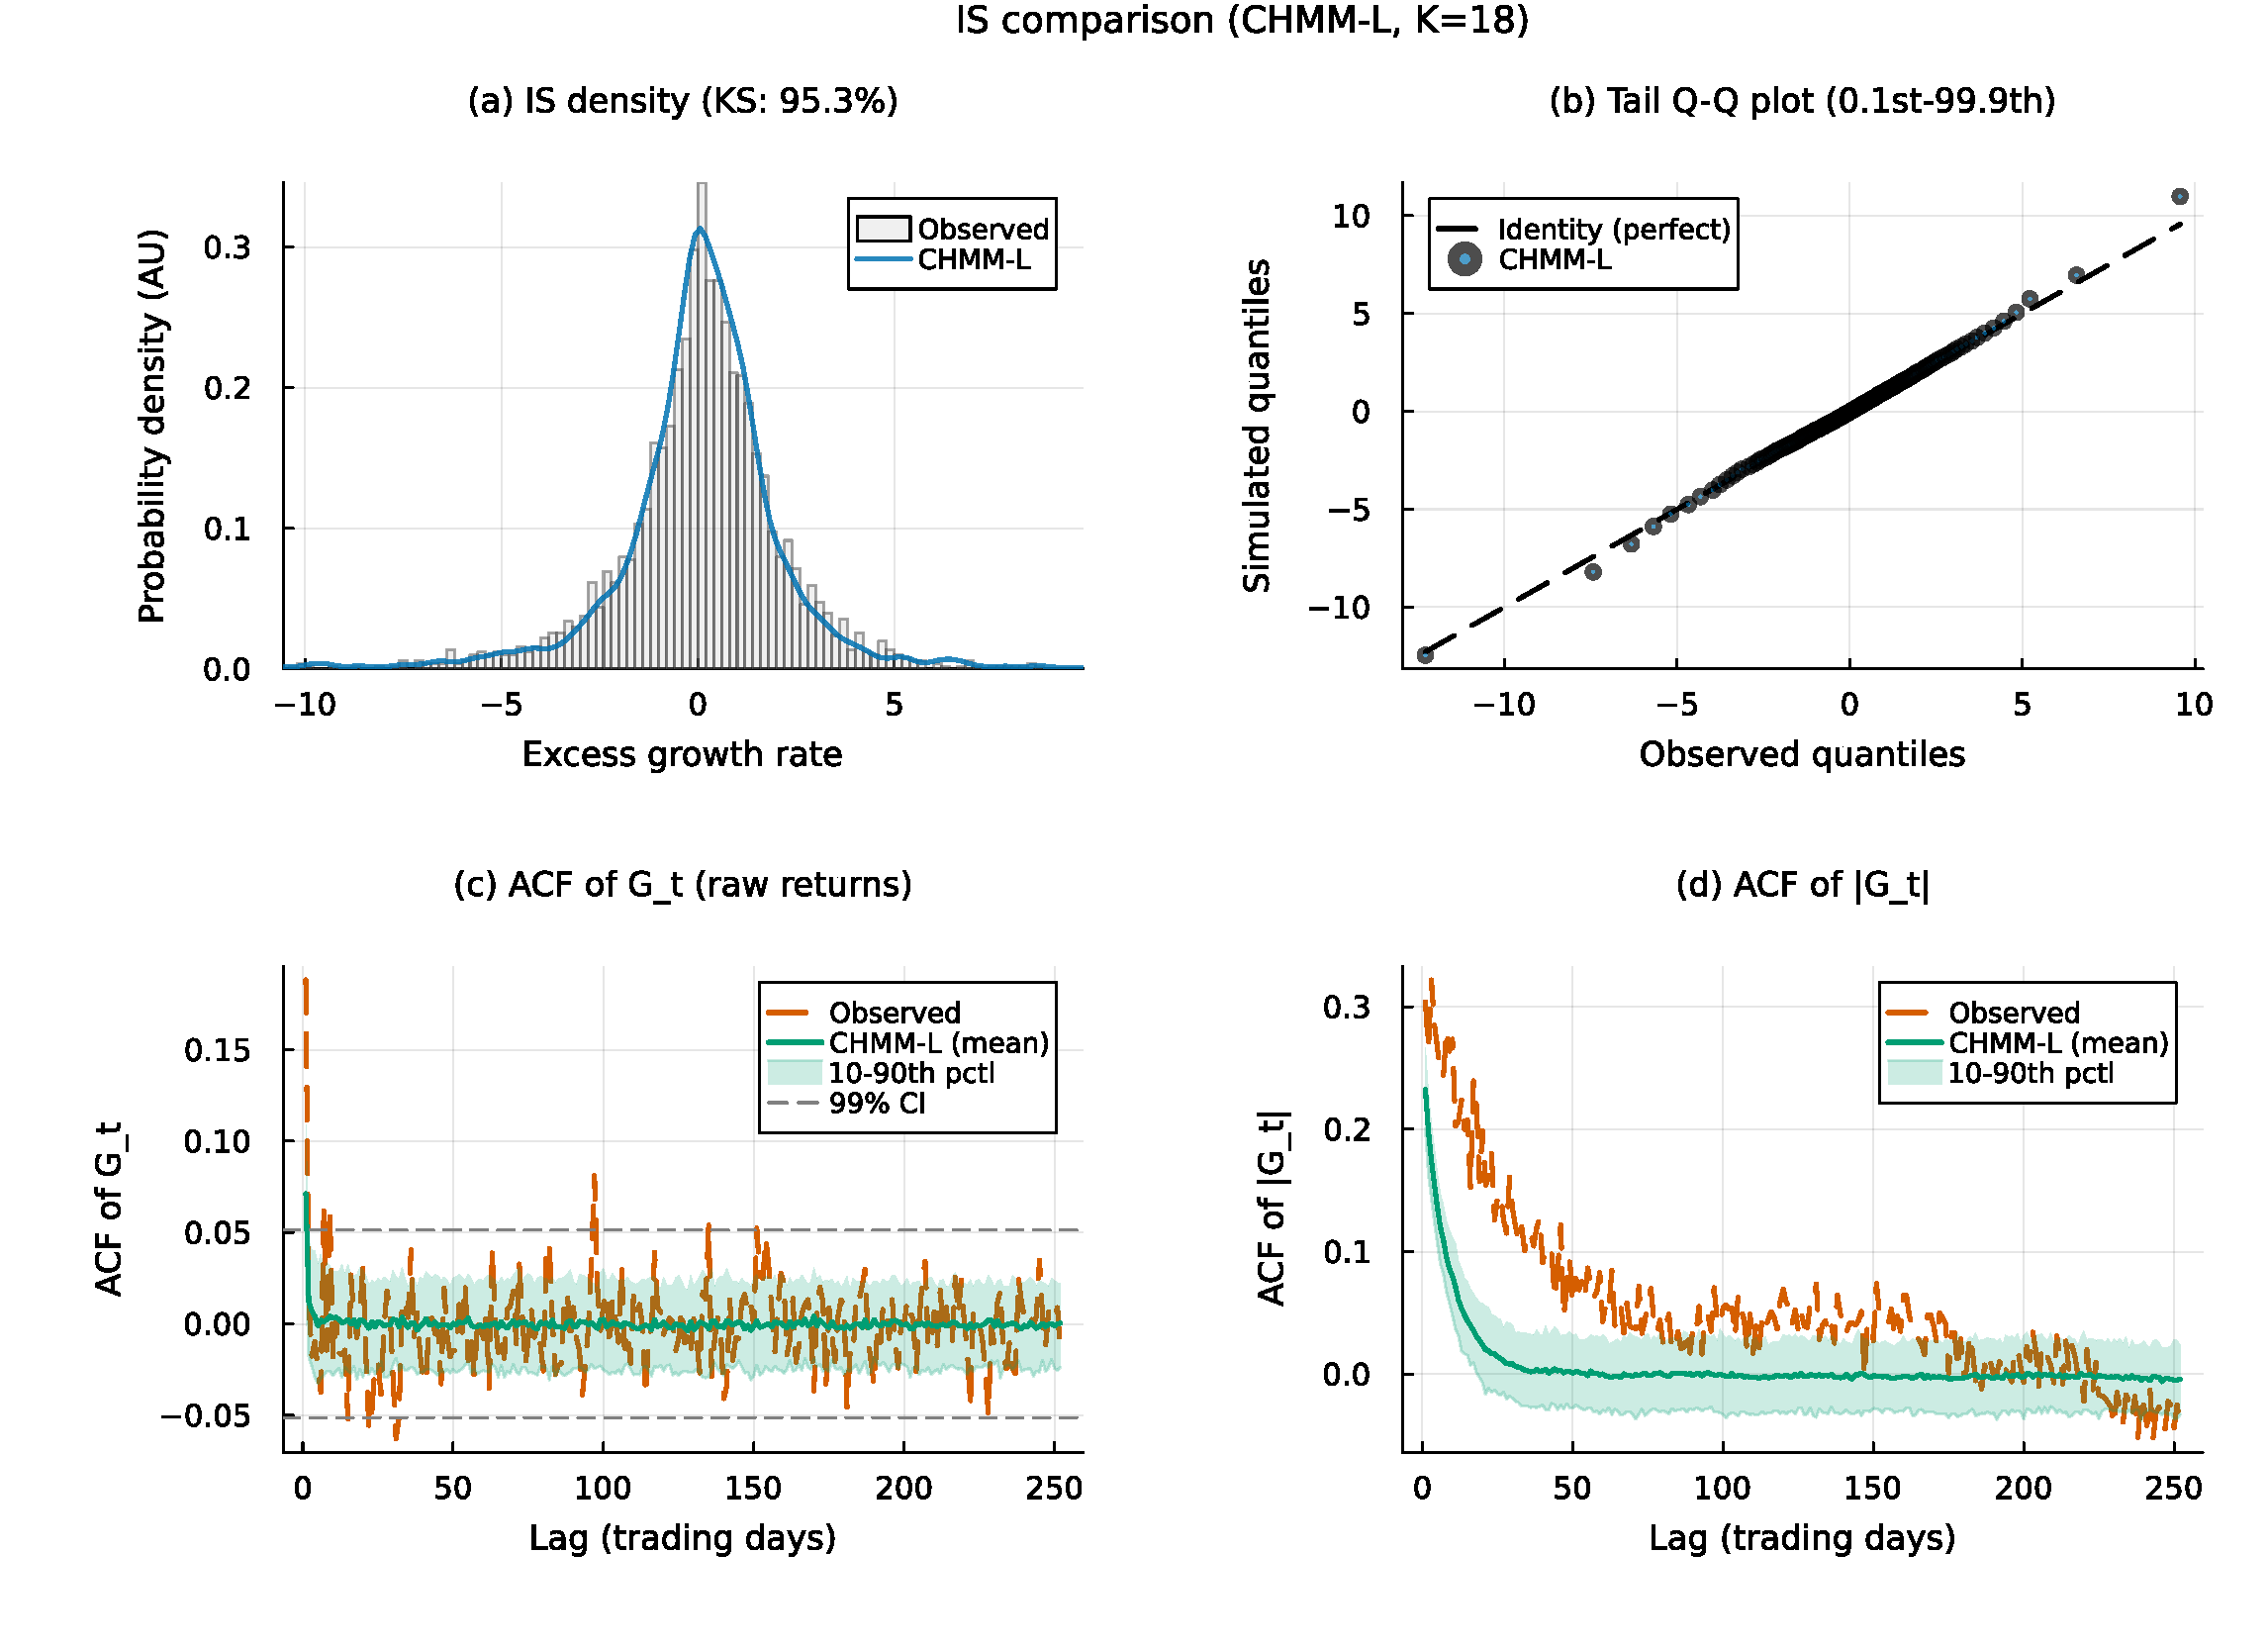
\includegraphics[width=\textwidth]{figs/Fig-3-IS-Comparison-K18-L.pdf}
\caption{IS SPY model comparison at $K = 18$ for CHMM-L Laplace emissions (Pipeline~A, 1{,}000 simulated paths). Panels as in Figure~\ref{fig:is_families}.}
\label{fig:is_families_L}
\end{figure}

\paragraph{OoS validation.}
Figures~\ref{fig:oos_families}--\ref{fig:oos_families_L} show the OoS validation panels for CHMM-t and CHMM-L at $K = 18$.
The CHMM-t panel demonstrates the OoS kurtosis alignment noted in the main text (simulated 6.40 vs.\ observed 6.24), and the CHMM-L panel shows the tighter density fan produced by the heavier Laplace tails relative to the Gaussian.

\begin{figure}[H]
\centering
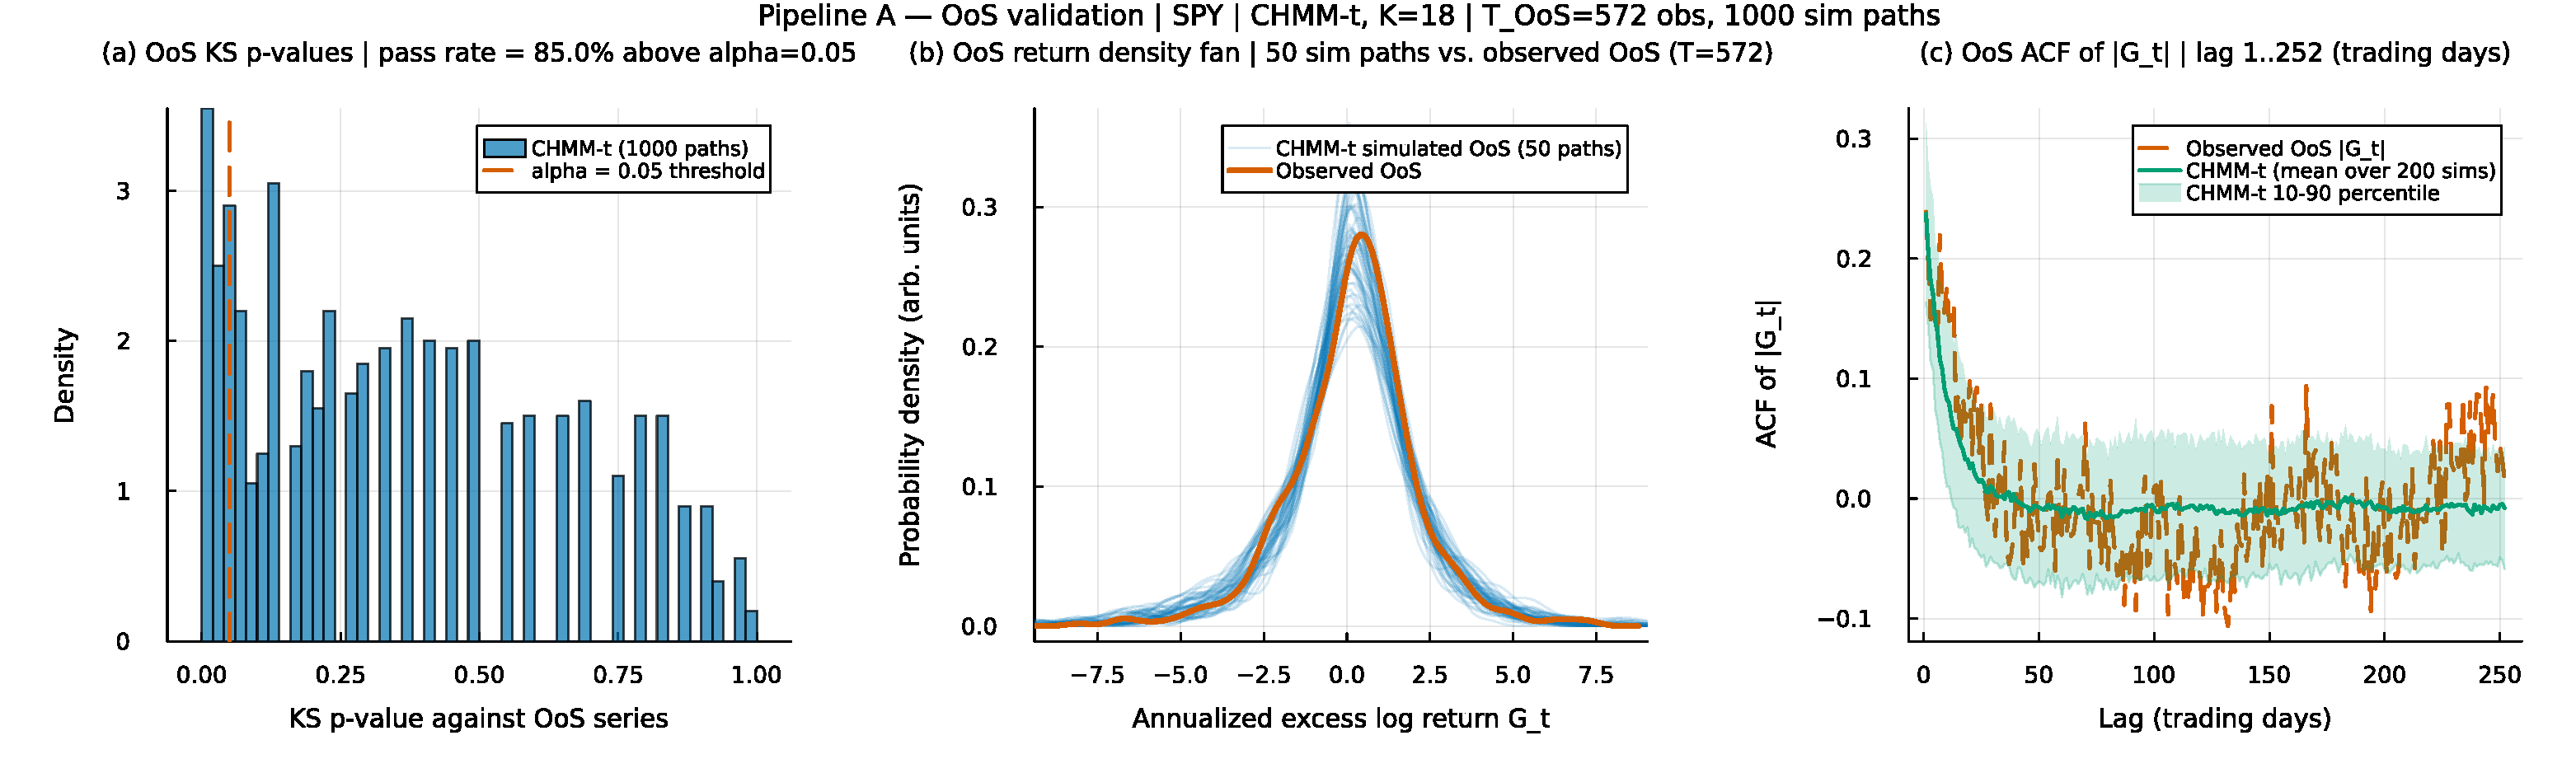
\includegraphics[width=\textwidth]{figs/Fig-4-OoS-Validation-K18-t.pdf}
\caption{OoS SPY validation at $K = 18$ for CHMM-t Student-t emissions (Pipeline~A, 1{,}000 simulated paths). Panels show (a) KS $p$-values, (b) OoS density fan, and (c) OoS ACF of $|G_t|$. The CHMM-N counterpart is Figure~\ref{fig:oos_validation}; the CHMM-L counterpart is Figure~\ref{fig:oos_families_L}.}
\label{fig:oos_families}
\end{figure}

\begin{figure}[H]
\centering
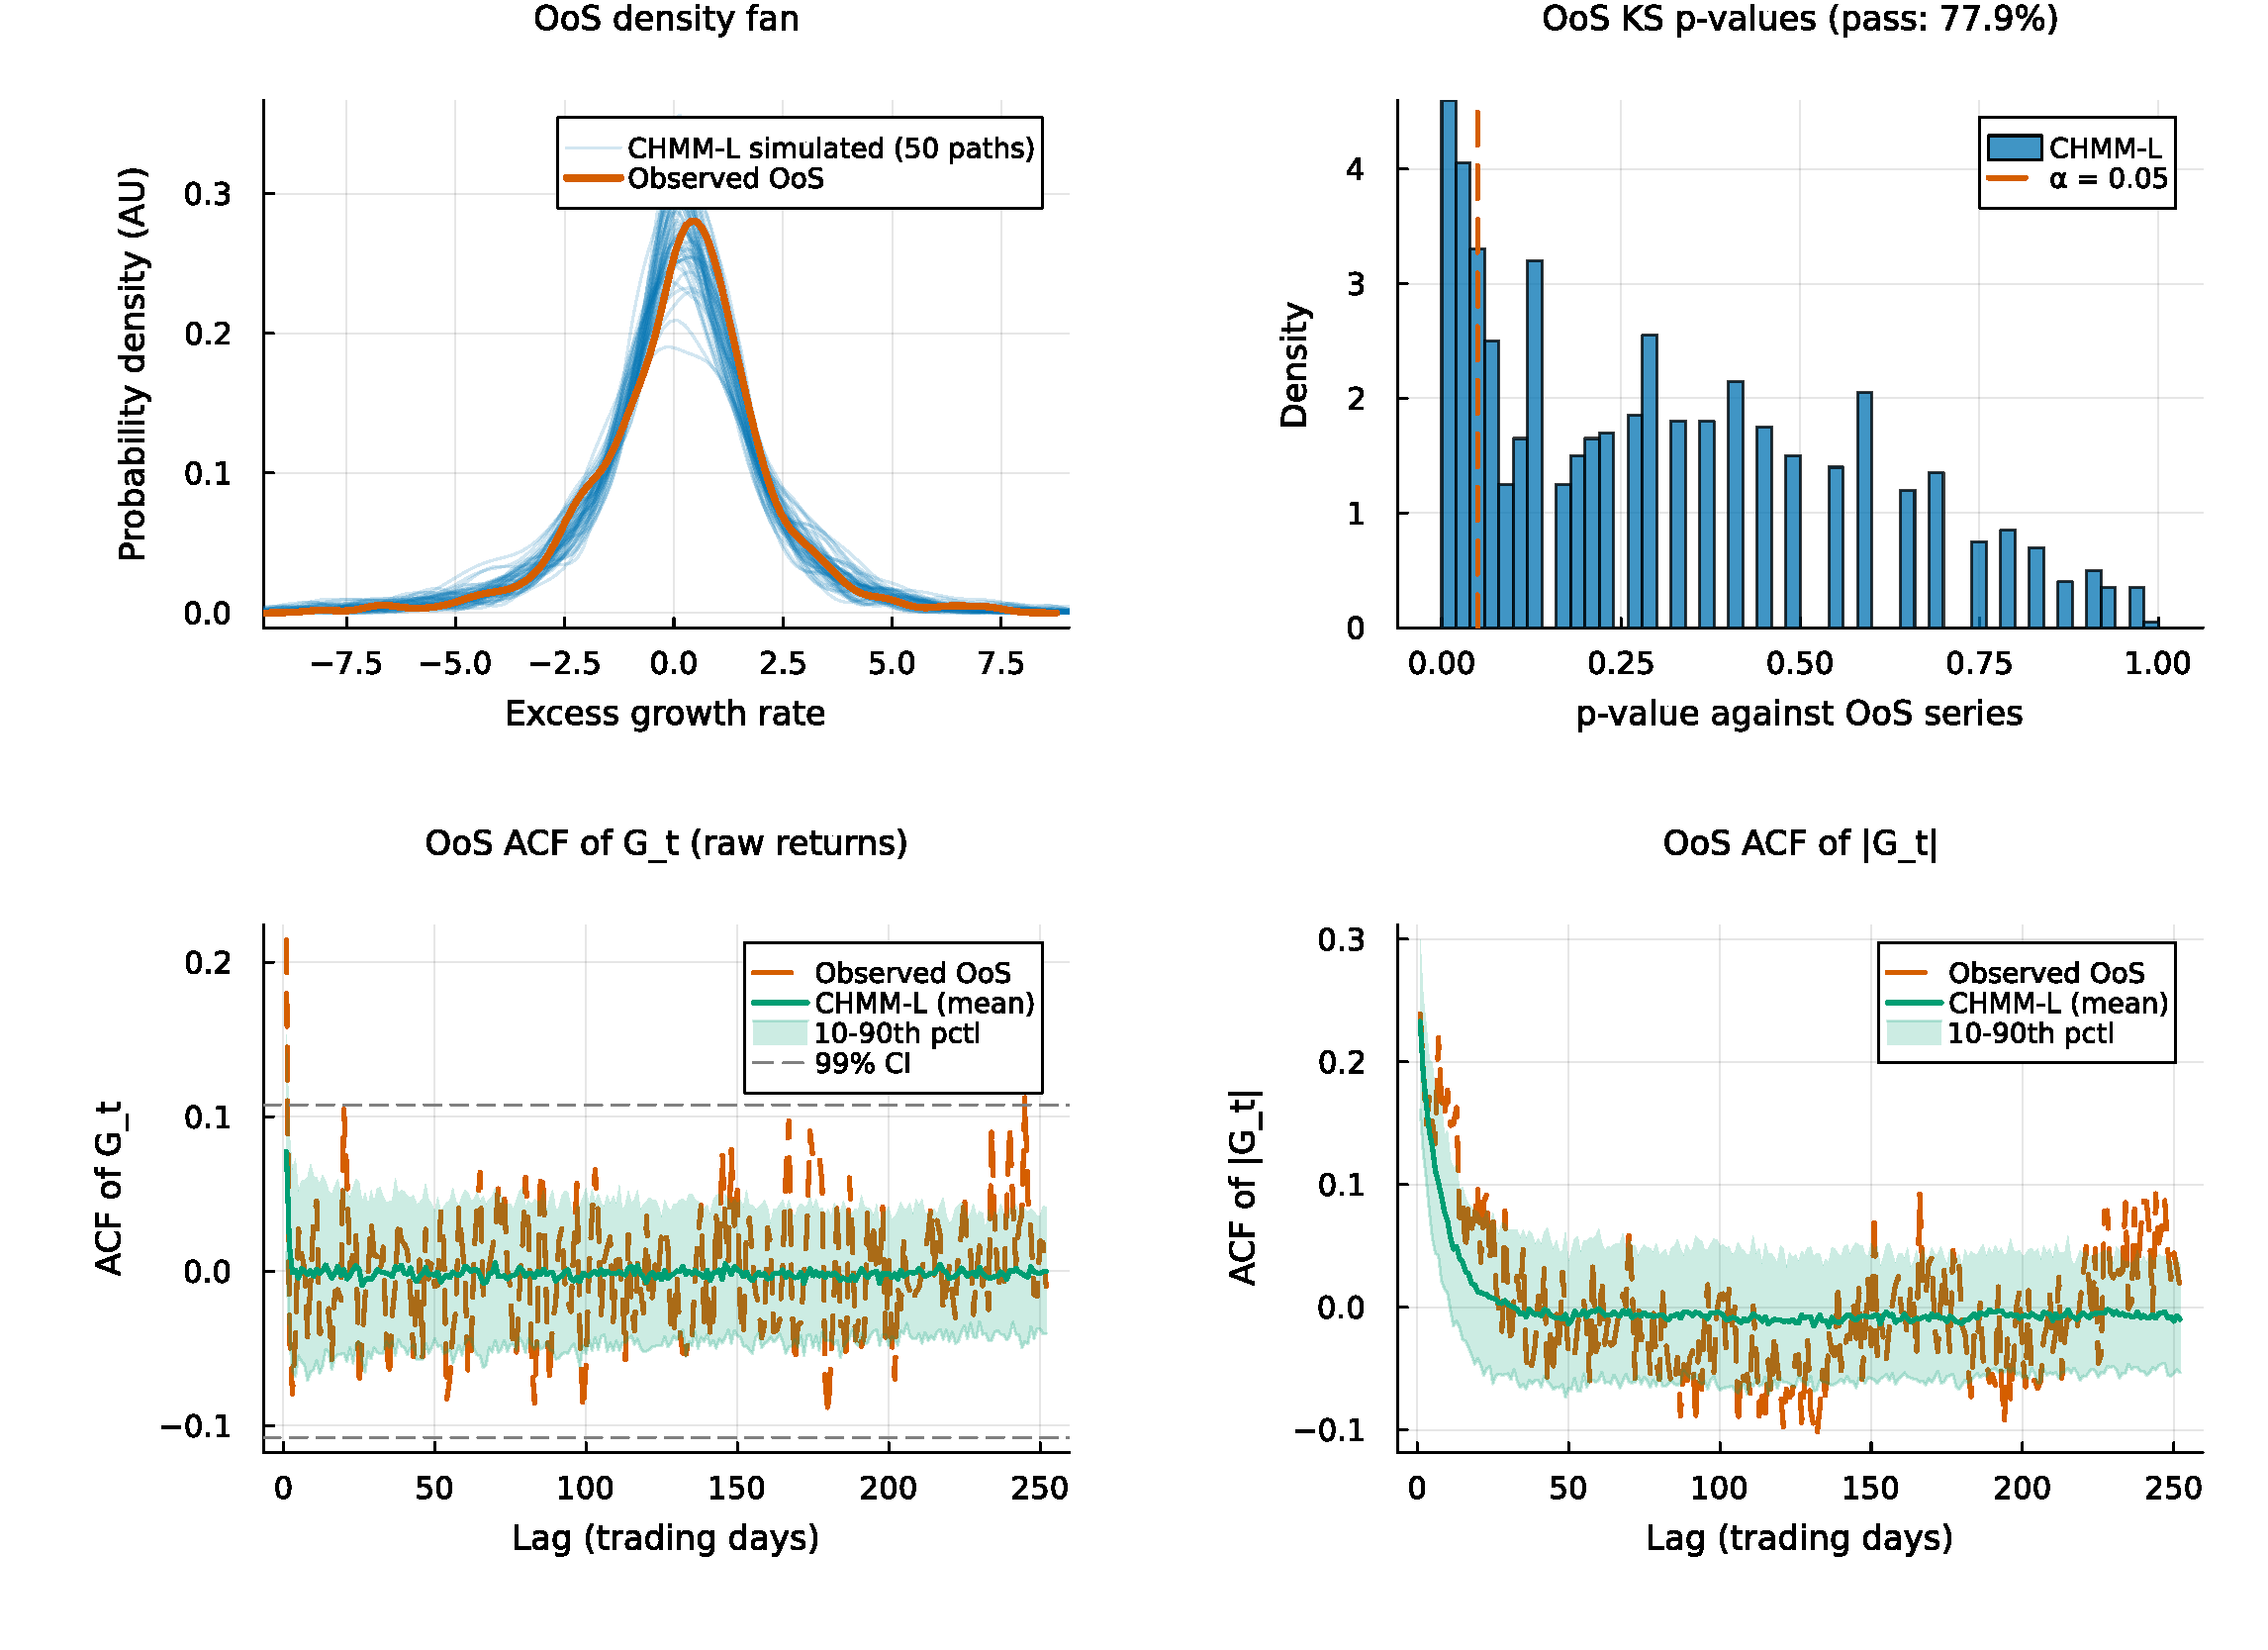
\includegraphics[width=\textwidth]{figs/Fig-4-OoS-Validation-K18-L.pdf}
\caption{OoS SPY validation at $K = 18$ for CHMM-L Laplace emissions (Pipeline~A, 1{,}000 simulated paths). Panels as in Figure~\ref{fig:oos_families}.}
\label{fig:oos_families_L}
\end{figure}

\paragraph{Convergence.}
Figure~\ref{fig:convergence_families} shows the Baum-Welch / ECM / weighted-EM log-likelihood histories at $K = 18$ for all three families.
The CHMM-t and CHMM-L curves inherit the monotone increase of the classical EM guarantee; the CHMM-t curve has a slightly longer pre-plateau phase because each ECM sub-iteration refines $\nu_k$ with a golden-section search.

\begin{figure}[H]
\centering
\begin{subfigure}[b]{0.32\textwidth}
    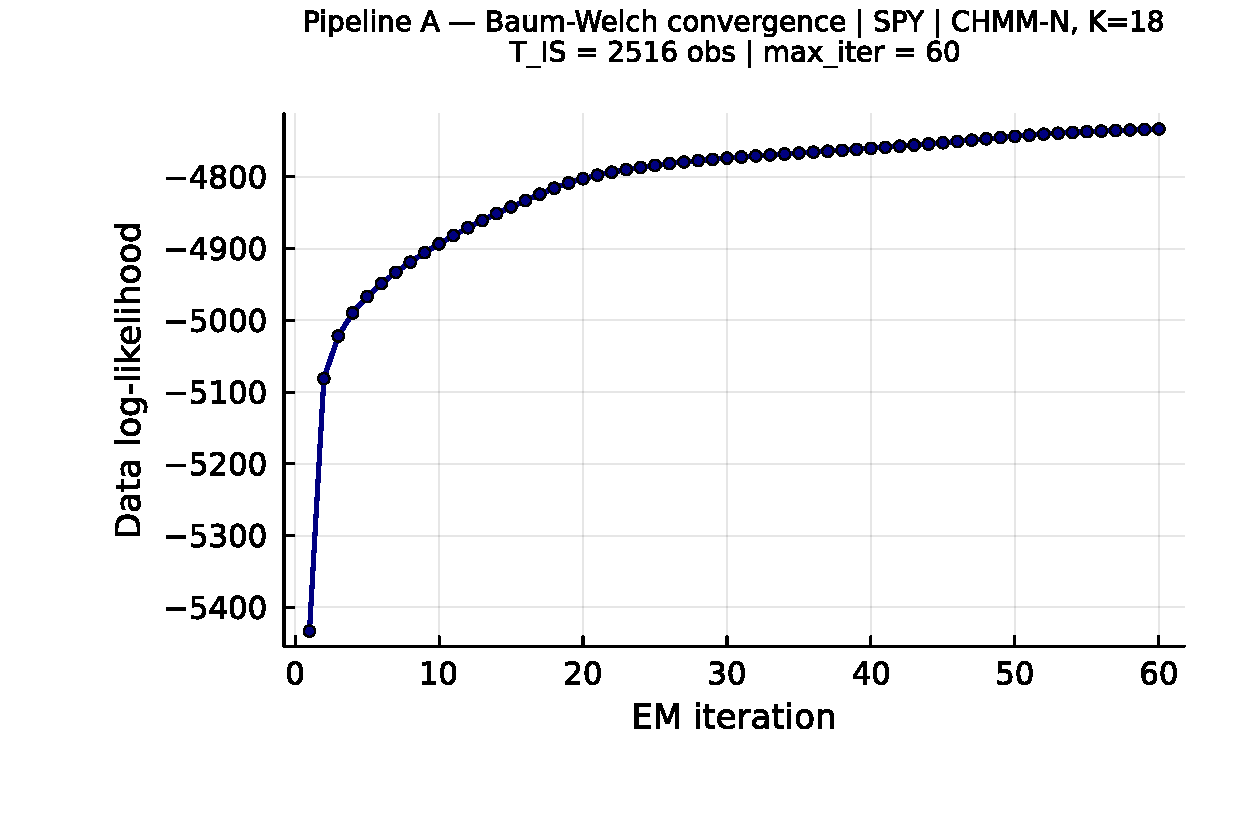
\includegraphics[width=\textwidth]{figs/Fig-Convergence-K18-N.pdf}
    \caption{CHMM-N}
\end{subfigure}
\hfill
\begin{subfigure}[b]{0.32\textwidth}
    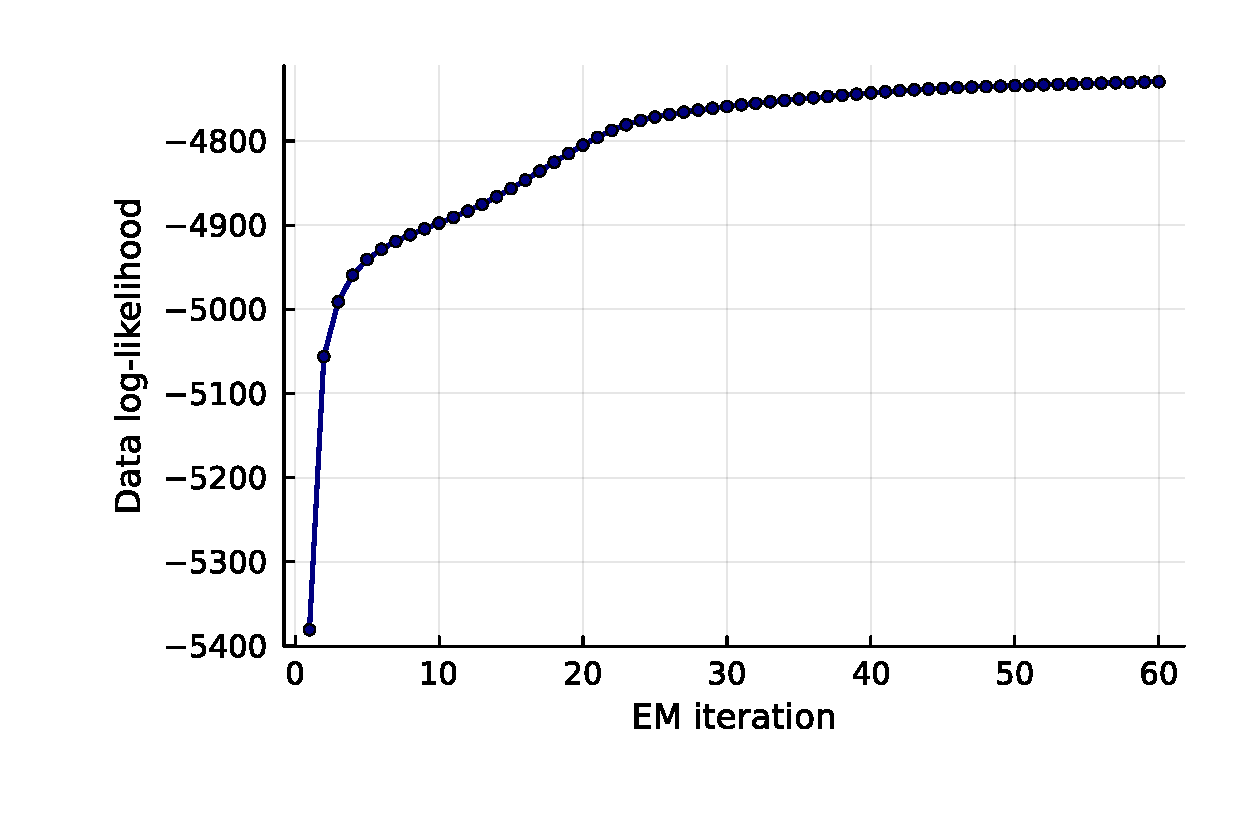
\includegraphics[width=\textwidth]{figs/Fig-Convergence-K18-t.pdf}
    \caption{CHMM-t}
\end{subfigure}
\hfill
\begin{subfigure}[b]{0.32\textwidth}
    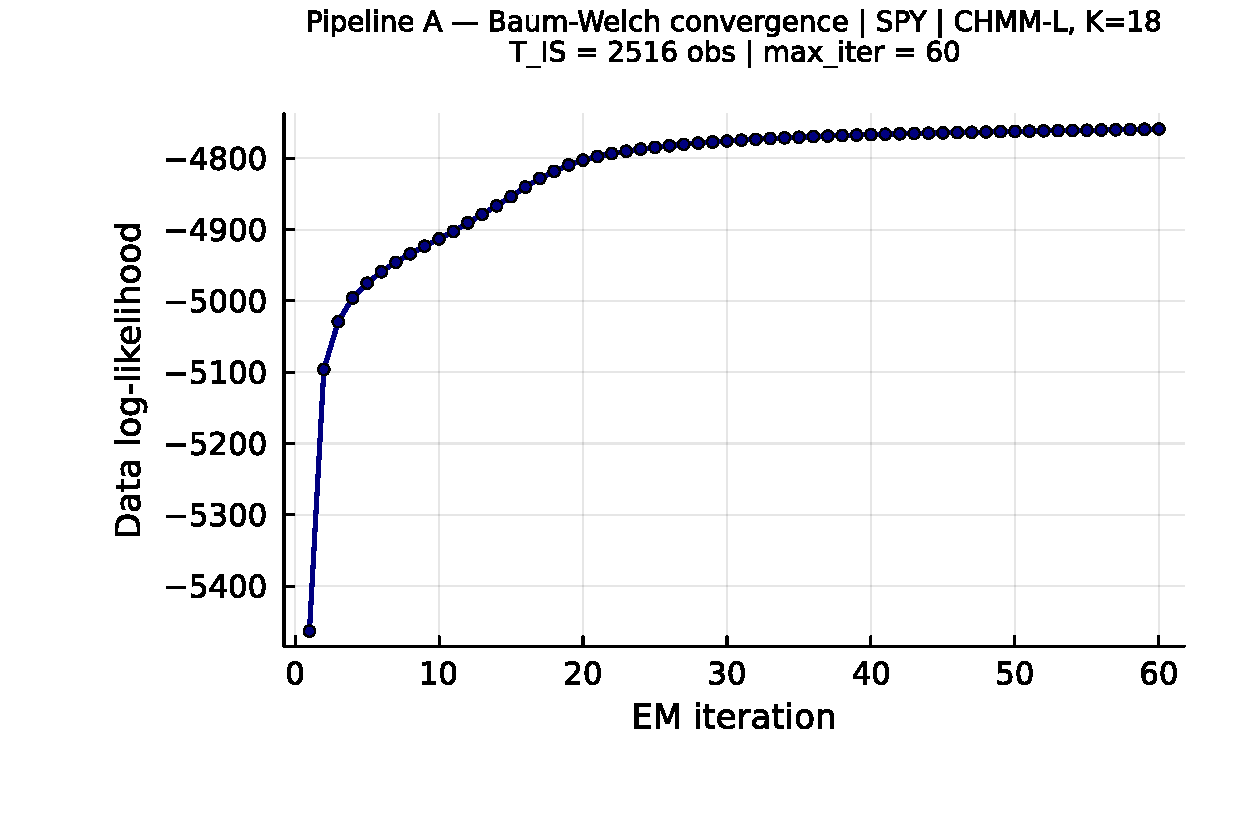
\includegraphics[width=\textwidth]{figs/Fig-Convergence-K18-L.pdf}
    \caption{CHMM-L}
\end{subfigure}
\caption{Log-likelihood histories for the SPY IS fit (Pipeline~A) at $K = 18$ across the three emission families (CHMM-N Gaussian classical EM; CHMM-t Student-t ECM with per-state $\nu_k$ golden-section sub-step; CHMM-L Laplace weighted-EM). All three curves are monotonically non-decreasing and plateau well before the $\texttt{max\_iter} = 60$ budget.}
\label{fig:convergence_families}
\end{figure}

\subsubsection{Ryd\'{e}n K = 2 Replication}
\label{sec:ryden_replication}

Table~\ref{tab:ryden_init} reports the direct replication of Ryd\'{e}n et al.'s 1998 $K = 2$ setting on SPY IS under both initialization strategies, as discussed in Section~\ref{sec:discussion}.
The quantile-based initialization used in the main body is row 1; five independent random-seed initializations are rows 2--6.
Random init here draws per-state $(\mu_k, \sigma_k)$ from a moderate perturbation of the sample moments, which is representative of the random-init practice common in the 1990s HMM literature.

\begin{table}[h]
\centering
\small
\caption{Ryd\'{e}n replication: $K = 2$ CHMM-N on SPY IS under quantile vs random initialization (seed sub-index varies the random init).}
\label{tab:ryden_init}
\begin{tabular}{l c c c c c}
\toprule
Init & KS IS (\%) & AD IS (\%) & ACF-MAE & Kurt IS & KS OoS (\%) \\
\midrule
Quantile (main body) & 79.0 & 71.5 & 0.0501 & 2.57 & 72.4 \\
Random seed = 1      & 78.7 & 70.7 & 0.0502 & 2.57 & 73.2 \\
Random seed = 7      & 75.3 & 69.6 & 0.0498 & 2.56 & 74.0 \\
Random seed = 42     & 77.6 & 70.0 & 0.0498 & 2.59 & 71.8 \\
Random seed = 100    & 76.2 & 69.4 & 0.0500 & 2.59 & 72.3 \\
Random seed = 2024   & 76.4 & 69.8 & 0.0499 & 2.54 & 72.9 \\
\bottomrule
\end{tabular}
\end{table}

The key observation is that ACF-MAE is essentially constant at $\approx 0.050$ across all six rows, matching the $K = 18$ CHMM-N of the main body.
IS KS pass rate remains below the $K = 18$ operating point ($75.3$--$79.0\%$) because two Gaussian components cannot tile the full multi-regime return distribution.
The combination is consistent with the reading that the binding low-$K$ constraint in the \citet{ryden1998stylized} setup is distributional rather than temporal: the ACF is already well reproduced at $K = 2$, and it is distributional fidelity that drives the preference for $K = 18$.

